
\documentclass[twocolumn]{article}
% {amsart}
\usepackage[top=0.75in, left=0.65in, right=0.65in, bottom=0.6in]{geometry}

\usepackage[utf8]{inputenc}

\usepackage{float}

% \usepackage{url}
% \usepackage{xurl}
\usepackage[pdftex]{hyperref}

% code sux, use "lstlisting"
%\usepackage{code}
\usepackage{listings}
% \usepackage{cite}
\usepackage{latexsym}
\usepackage{amsmath}
\usepackage{amssymb}
\usepackage{graphicx}
% IPA symbols. safe turns off overrides for like \! which I still want
% \usepackage[safe]{tipa}
\usepackage{chessboard}
\usepackage{supertabular}
\usepackage{enumitem}

% Put a line under figure captions, to better separate them from
% the text.
\usepackage{caption}
\DeclareCaptionFormat{tomlinesep}{#1#2#3\hrulefill}
\captionsetup[figure]{format=tomlinesep}

% \usepackage[most]{tcolorbox}

% lets me explicitly set a. or 1. etc. as enum label
% \usepackage{enumitem}

\pagestyle{empty}

\usepackage{ulem}
% go back to italics for emphasis, though
\normalem

% do "fancy" stuff like verbatim in footnotes
\usepackage{fancyvrb}
\VerbatimFootnotes

\usepackage{natbib}
\setcitestyle{numbers,square}

\interfootnotelinepenalty=0
\setlength{\footnotesep}{2em}

% \startsquarepar and \stopsquarepar allows justifying the
% whole paragraph, including its last line
\newcommand{\startsquarepar}{%
    \par\begingroup \parfillskip 0pt \relax}
\newcommand{\stopsquarepar}{%
    \par\endgroup}

% Style for code listings.
\lstdefinestyle{codestyle}{
  basicstyle=\ttfamily\footnotesize,
  breaklines=false,
  keepspaces=true,
}

\lstset{style=codestyle}

\newcommand\sfrac[2]{\!{}\,^{#1}\!/{}\!_{#2}}
\newcommand\xbyx[2]{\ensuremath{#1 {\times} #2}}
\newcommand\basis{\ensuremath{\textrm{\bf b}}}

\renewcommand\comment[1]{}

% XXX the collection of crap above causes a first page
% with just "1" on it (probably conflicting packages). This
% magic just drops the first page, which is of course not
% the right solution, but...

\usepackage{atbegshi}% http://ctan.org/pkg/atbegshi
\AtBeginDocument{\AtBeginShipoutNext{\AtBeginShipoutDiscard}}

\begin{document}

\title{GradIEEEnt half decent}
\author{Dr.~Tom~Murphy~VII~Ph.D.}\thanks{
Copyright \copyright\ 2023 the Regents of the Wikiplia Foundation.
Appears in SIGBOVIK~2023 with the
signaling NaN
of the Association for Computational Heresy; {\em IEEEEEE!}
press, Verlag-Verlag volume no.~0x40-2A. 1 ULP
}

\renewcommand\th{\ensuremath{{}^{\textrm{th}}}}
\newcommand\st{\ensuremath{{}^{\textrm{st}}}}
\newcommand\rd{\ensuremath{{}^{\textrm{rd}}}}
\newcommand\nd{\ensuremath{{}^{\textrm{nd}}}}

\newcommand\gradone{{\sf grad1}}
\newcommand\downshifttwo{{\sf downshift2}}
\newcommand\plussixtyfour{{\sf plus64}}

\renewcommand\paragraph[1]{\smallskip \noindent{\bf #1}\enspace}

\date{0 April 2023}

\maketitle \thispagestyle{empty}

\sloppypar


\section{Introduction}



Imagine you are my professor. Maybe you actually were my professor, in
which case you may already be sweating before I say any more. The
subject matter is Neural Networks. You draw the

``Now this transfer function can be almost anything. Typically it
would be something like the hyperbolic tangent, which looks like this.

\begin{center}
\includegraphics[width=0.75 \linewidth]{tanh}
\end{center}

``But it has to be a non-linear function. If it's linear, i.e.~of the
form $y = mx + b$, then observe that the entire layer is a linear
function. And so the entire network is just a linear function of
linear functions; itself a linear function. We could just compute an
equivalent single-layer network, and we know that it could only fit
linear functions, which is insufficient for most problems.''

Then I raise my hand. The speed with which I raise it, and the subtle
forward pose of my arm suggests that I want to pluck an abstract idea
from the whiteboard and pervert it. You know this look, and you're
reluctant to call on me. But no other students are asking questions.
You must call on me.

``Tom.'' It's more like a statement then a question. It includes the
tone of spoken punctuation that, if it could, ends the entire
conversation before it begins.

``OK but, when we implement this on a computer we'll use some
approximation of numbers, like floating point. So the specific
sequence of additions and multiplications will matter. It's not
actually equivalent to rearrange them to a single layer because you
don't have distributivity, commutativity, etc.''

``Uh. I think that's technically true, but for all practical purposes \ldots''

``What about *im*practical purposes?''

You vigorously strangle me, and I die.

$\bigskip$
$\cdots$
$\bigskip$

That was about 20 years ago. The world will not let us stop thinking
about neural networks. And so this question has been on my mind for a
long time. Just to be clear, the professor was right: This is not an
important question. Theoretically I am right, but for practical
purposes it probably does not matter. But I like to work at the
intersection of Theory and Impractice. We can make it matter by doing
a lot of work. And then I will continue to be right theoretically, but
also more right because it will only matter for {\em most} practical
purposes.

So this paper is an exhaustive exploration of what we can do with just
floating point addition and multiplication by constants (scaling). You
should only be able to make lines, but I'll demonstrate that due to
rounding error, you can absolutely use ``linear'' transfer functions
in neural networks. Machine learning is not the only field with a
proclamation that some function must be ``non-linear,'' so we'll look
at a few of those as well. There will of course be several hearty
digressions. By studying these functions we'll see that they are
almost arbitrarily rich, and conclude with a demonstration of their
completeness in the field of Plumbing.

TODO intro: We'll develop a better understanding of where floating point inaccuracy comes from, and how to get it quickly, and how to use it for our benefit.

\section{A refresher on neural networks}
Let's repeat the professor's lesson. This section is easily skippable
if you are a plucky student who thinks they already know everything.
At a high level, a NN is a way of implementing a numeric function
(takes a bunch of numbers as input, and gives a bunch of numbers as
output). The network consists of a number of {\it layers}, where the first
layer is the input and the last layer is the output.

TODO DIAGRAM

The numbers that fill in each layer are its {\it activations}. Each
layer's activations are computed from (just) the previous layer,
according to a formula:

$$a_i = TF(w_{1i} * p_1 + \ldots w_{ni} * p_n + b_i)$$

Where $p_j$ is the activation of the $j$th node on the previous layer,
and $w_{ji}$ is the weight parameter, and $b_i$ is the bias parameter.
The weight and bias parameters are learned during the training of the
neural network, but just become constants when using the NN to compute
its output.

$TF$ is the transfer function, which is of particular interest in this
project. Classically, the transfer function was some kind of sigmoid.
The {\tt tanh} function pictured in the introduction is a good example
of a sigmoid. The intuition behind this is that, thinking about $a_i$
as some kind of neuron, the neuron ``fires'' (activates) with some
probability. This probability gets higher as its input values get
larger (but note that weights can be negative, so upstream neurons can
also have an inhibitory effect). But since it is a probability, the
% XXX ok but tanh actually outputs [-1,1]
value must be in [0, 1]; the transfer function ensures this.

\paragraph{Differentiability.}
Another important property of the transfer function is that it be
differentiable, because the stochastic gradient descent algorithm used
to train NNs needs to be able to move along some error-reducing
gradient, and back-propagate errors to earlier layers. This gradient
is just the derivative of the function.

\paragraph{What transfer functions ought to exist?}
We used to think that these saturating transfer functions were ideal.
But this turns out to be wrong, especially for internal (``hidden'')
layers. Transfer functions don't need to produce probabilities, and
they can have unbounded range. A wide variety of functions will work,
including extremely simple ones. The most popular transfer function in
2023 is the ``rectified linear unit,'' which looks like this:

\begin{center}
\includegraphics[width=0.33 \linewidth]{relu}
\end{center}

This one is extremely easy to implement (\verb+x < 0 ? 0 : x+), is fast
and seems to work very well, possibly because its derivative is
significant (one) on the entire positive side. (In contrast, sigmoids
tend to get ``stuck'' because of their saturating behavior; their
derivatives become nearly zero.) Note that it is not actually
differentiable (discontinuity at zero) but ``for all practical
purposes'' it is differentiable.

The (only?) apparently essential quality of the transfer function is
that it be non-linear. If it is instead of the form $TF(x) = mx + b$,
then $a_i$ is also just a linear function of the previous layer, as
linear functions of linear functions (weighted sum) are linear. This
causes the entire NN to be a linear function. It is well known that a
linear function ``cannot'' represent some other simple functions, such
as XOR.

$$\nexists m,n,b.\,\, XOR(x, y) \approxeq m x + n y + b$$
% FORMULA: Not exists m n b, such that $XOR(x, y) \approxeq m x + n y + b$

This means that with a linear transfer function, a NN could never
learn even a simple function like XOR. Many problems we want to learn
are in fact much more complicated.

\section{A fine terminological issue}
affine vs linear

(Here we need to clarify exactly what operations we allow!) THE RULES


\section{Half-precision IEEE-754 floating point}
In this project we'll abuse floating point inaccuracy to create
``linear'' functions (only using floating point addition and scaling)
that are not lines. For this reason, we prefer to have a numerical
system that is {\em less accurate}. In floating point, inaccuracy comes
from the fact that not all numbers are representable (due to finite
precision) and the result of an operation is always rounded to a
representable number. IEEE-754 floating point comes in different
``spice levels,'' with ``32-bits'' being ``float'' and ``64-bits''
being ``double.'' Although spice levels as low as 3 bits make
sense~\cite{murphy2019nan}, 8-bit (``mild'') is occasionally used in
real applications, and 16-bit (``half'') is quite common in machine
learning. Usually the reason to prefer half precision is that it uses
less memory, and so your GPU can store networks that are twice as big
in RAM. For this project we will also use half precision, and we will
be happy to save RAM, but more happy that its precision is low and so
it is practical (although silly) to achieve significant rounding
error. Another important reason to choose half precision is to make
the pun in the title.

A half precision float is 16 bits: One sign bit, five bits for the
exponent, and 10 bits for the mantissa. Like all IEEE-754 formats,
there is much more precision (more values are representable) near
zero. (Figure~\ref{fig:histogram}) Once you get to 1024,
only integers are representable. From 2048 to 4096, only even numbers
are representable. 65504 is the largest finite number, and up here,
only multiples of 32 are available.

\begin{figure}
FIGURE: HISTOGRAM
\caption{
Here I will put a histogram of the values.
  } \label{fig:histogram}
\end{figure}

Some CPUs have native support for half-precision IEEE, but typically
via non-standard intrinsics or compiler flags. Since people using
half-precision are usually doing so in the interests of performance,
many configurations will ``help'' you by performing practical but
incorrect optimizations. This is similar to what happens when enabling
\verb|--ffast-math|, which stands for Final Fantasy AST Math, meaning
that the abstract syntax tree of your program will be manipulated
using fantasies about Math that do not apply to IEEE-754, and your
Final result can be arbitrarily different. For the ideas in this paper
to work, \verb|--ffast-math| is prohibited. And it will be slow!

Rather than deal with non-standard stuff, I found a nice library
called {\tt half.h}~\cite{half} that implements IEEE-754 compliant
half-precision in portable C++. I use this throughout the project
and it matches the behavior of my GPU. I recommend it for similar
hijinks.

% Where does floating point imprecision come from?
\paragraph{Origins of Imprecision.}
Floating point does have many perversions, but many programmers come
to believe all sorts of dangerous superstitions about it. One idea is
that floating point is somehow always inexact, and so that you always
have to check that two numbers are equal ``within some
epsilon''~\cite{murphy2014epsilon}. This may work ``in practice'' but
it is actually pretty sloppy. Floating point imprecision is not
random, nor is it constrained to a fixed epsilon. Operations are
defined much more usefully: Each one computes the mathematically
correct value, and then rounds (according to the ``rounding mode'') to
the nearest representable value. That's it. One consequence of this is
that you can get the exact result of 32-bit multiplication by doing
64-bit multiplication and then rounding to 32 bits. This also means
that the rounding error from a single operation can be as large as the
gap between representable numbers: Up to 32 for half-precision. But it
also means that operations whose results can be exactly represented
have no error; for example adding integral half values less than 512
will always give an exact integer result, which can be compared using
==. We will use this later in Section~\ref{sec:fluint}. It is
neither necessary nor sufficient compare for ``equality'' with some
``epsilon.''

\paragraph{Rounding.}
IEEE-754 supports multiple rounding modes, like ``round-to-zero,'' and
``round-to-infinity'' (always round in the positive direction).
Throughout this paper we use ``round-to-nearest,'' which is also the
typical default (e.g.~for C++11 expressions evaluated at compile time,
it always uses round-to-nearest).\footnote{There is seldom reason to
  change the rounding mode, and since it is a stateful act, you're
  asking for it if you do. But the round-to-negative-infinity and
  round-to-positive-infinity modes are are useful for interval
  arithmetic, which is arguably the only truly reasonable way to use
  floating point. What you do is represent numbers as intervals (low
  and high endpoints) that contain the true value, and then perform
  each calculation on both endpoints. For computations on the low
  endpoint, you round down, and symmetrically for the high endpoint.
  This way, the true value is always within the interval, and you also
  know how much inaccuracy you have accumulated!} Similar results are
likely attainable for the other rounding modes, as well as
hypothetical rounding modes such as ``round away from nearest,'' but I
have not explored this.

\paragraph{Getting some nonlinearity.} \label{sec:plus128}
All transfer functions implemented with floating point have a finite
range. For our experiments with neural networks, we will focus on
transfer functions that map values in [-1, 1] to values in [-1, 1].
Almost half (48.4\%) of floating point values are in this interval and this
is a typical nominal range for activations in neural networks.

We only have two operations: Addition and scaling. Let's see what kind
of rounding error each of these gives us. First, addition. In order to
get a function that takes values in [-1, 1] to values in [-1, 1], we
want to first add a constant (giving us perhaps a large value) and
then add a negative constant, bringing us back in range. For example,
the constant 128 gives us the function

$$f(x) = x + 128.0 - 128.0$$

This is of course mathematically the same as $f(x) = x$ (the
identity), but with half precision we get a function that looks like
this

\begin{center}
\includegraphics[width=0.45 \linewidth]{plus128}
\end{center}


Between 128 and 256, only multiples of 0.125 are representable. So for
arguments in 0 to 1, the sum is rounded to one of the values 128.0,
128.125, 128.25, \ldots 129. From 64 to 128, multiples of .0625
($\sfrac{1}{16}\th$) are representable. So from -1 to 0, we get 127.0, 127.0625,
127.125, \ldots 128. Subtracting 128, all of the values are exactly
representable, giving us -1, -.9375, \ldots, -0.0625, 0, 0.125,
\ldots, 0.875, 1.

The result is a step function, but whose resolution is twice as high
for the negative range as the positive; had we added -128 and then
added 128, we would have seen the opposite bias in resolution. We can
easily see that this function is (computationally) ``non-linear''
despite being (mathematically) ``linear.'' This function is unlikely
to be a good transfer function, because it does not have a good
derivative: It's zero most places (flat segments) except at the
discontinuities, where it is undefined. We do test this approach
(with the constant 64.0) later, though.

Scaling gives similar results. Consider

$$f(x) = x * 100.0 * (1.0 / 100.0)$$

In this project we never actually divide (although this would not
violate linearity) since most floating point numbers have approximate
multiplicative inverses, and many are exact. We just compute the
reciprocal $\sfrac{1}{100} \approxeq 0.01000213623$ ahead of time and
multiply by that constant. Here's what that function looks like:

\begin{center}
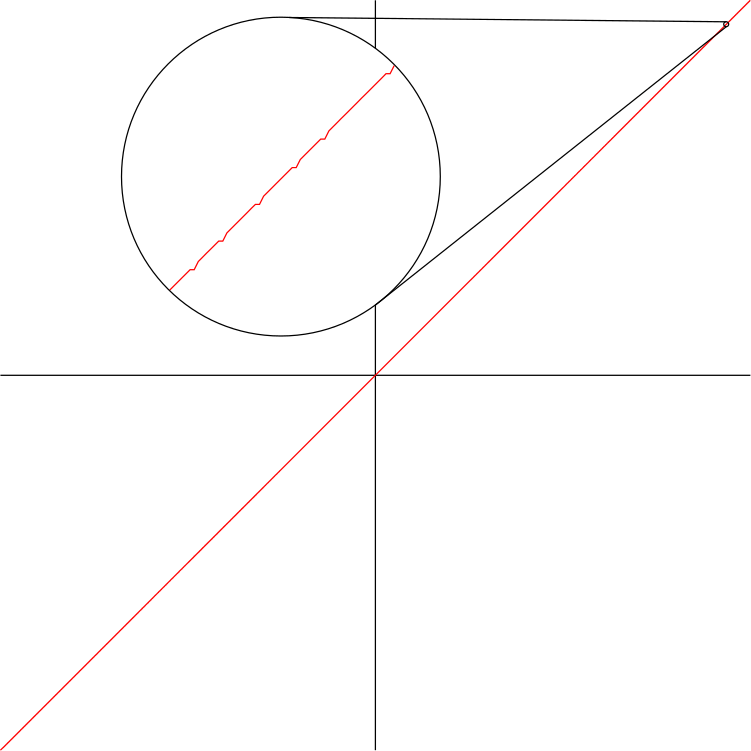
\includegraphics[width=0.45 \linewidth]{times100zoom}
\end{center}

At this scale it appears linear, but it does have small imperfections
(see zoomed region). The function is symmetric about zero, since
multiplication will do the same thing to a positive number as it does
to its negative counterpart. Here, the roundoff error differs with the
magnitude. At inputs close to 1.0, the results of the first
multiplication must round to the nearest multiple of 0.0625 (as in the
additive example) but this error is scaled down by a factor of 100
when we multiply back to the [-1, 1] range. So it is almost invisible.
For inputs close to 0.0, the error approaches zero. The effect is complex
and depends on the constant we multiply by. For example, if we multiply
by a power of two, this only affects the exponent, and so the result is
exact.

\medskip
Is that it? Of course not! We can apply these operations in
combination, and many times, to create more interesting functions. The
best approach I found in this simple family is to repeatedly multiply
the input by a number very close to one. Here's what happens if you
multiply the input by $0.99951171875$ (which is the next number
smaller than one, equal to $1 - \sfrac{1}{2048}$) five hundred times,
and then scale back at the end:

\[
\begin{array}{rcl}
  f(x) & = & x * (1 - \sfrac{1}{2048}) * (1 - \sfrac{1}{2048}) * \ldots \textrm{500 times} \ldots * \\
  \, & \, & 1.3232421875$$
\end{array}
\]

\begin{center}
\includegraphics[width=0.85 \linewidth]{grad1}
\end{center}

I call this the \gradone\ function.

Multiplying $1.0$ by $(1 - \sfrac{1}{2048})$ five hundred times in
half precision yields $0.755859375$ (mathematically it would be $(1 -
\sfrac{1}{2048})^{500} = 0.78333$, so there is significant accumulated
error. We set $f(1.0) = 1.0$ by multiplying by the inverse of this
constant, which is $1.3232421875$.

\begin{figure}[tp]
  \includegraphics[width=0.95 \linewidth]{rainbow} \\[1em]
  \includegraphics[width=0.95 \linewidth]{rainbow-error}
  \caption{
    How repeatedly multiplying by $1 - \sfrac{1}{2048}$ affects values in
    [0, 1].
    The width of the image is the interval [0, 1], with zero at the left.
    \\[1em]
    {\bf Top}: In the topmost row, we assign each pixel a hue so that
    we can track where those values go. For each pixel, we
    successively multiply by the constant and plot its color in its
    new $x$ position, the move to the next row down. Note that the
    rainbow shrinks exponentially as expected, but not smoothly.
    The black line is 500 iterations.
    \\[1em]
    {\bf Bottom}: The accumulated error when iteratively multiplying
    by the constant. Here the $x$ coordinate of the value does not move
    (so the middle column always represents the value that was
    originally 0.5). The color illustrates the accumulated error. For
    green pixels, the value is too high compared to the mathematically
    correct one; for magenta pixels too low. By choosing a row with
    alternations between green and red, we get the zig-zag pattern of
    the \gradone\ transfer function.
  } \label{fig:rainbow}
\end{figure}

Why does this result in the zig-zags? Multiplication by $(1 -
\sfrac{1}{2048})$ affects numbers differently. For constants less than
$6.1094760895 \times 10^{-5}$, the value is unchanged; we round back up to
the original value. For all other finite inputs it produces a smaller
value, but with rounding error that depends on the value. This error
accumulates and becomes significant with many iterations
(Figure~\ref{fig:rainbow}). Unlike the previous functions, the output
here is much smoother (it looks piecewise-linear); in each of these
segments its derivative is nondegenerate. Of course, this function is
mathematically linear. It is equivalent to $f(x) = x \times 1.036535$.

So now we have a ``good'' candidate function, which we'll call \gradone.
It is ``good'' in the sense that it is computationally non-linear
despite being mathematically linear, so it may prove my professor
wrong. On the other hand, it requires 501 floating point
multiplications to compute, which is kind of slow. The ``good'' news
is that since there are only 65536 16-bit values, we can easily just
precompute any function for all possible half inputs, and store it in
a table of 131072 bytes. This allows us to execute the function
efficiently when performance is important, such as during training.
(Table lookup is certainly not a mathematically linear operation, so
when we require the computation to be linear for ideological purposes,
we can perform the 501 multiplications and get the same result.)

\paragraph{Differentiating.}
Speaking of training, in order to train a neural network using
stochastic gradient descent, we need to be able to evaluate the
derivative of the transfer function at any point.
 XXX TODO EXPLAIN IT

\subsection{Bonus digression: Downshift}
Having freed myself from needing to ``do math'' in order to
differentiate exotic functions, I pondered other weird transfer
functions. For example, the rectified linear transfer function is very
simple and works well, but is it the fastest possible transfer
function that might work? It does involve a conditional, which na\"ively
implies comparison and branching (although probably most processors
can do this with a conditional move). Because the floating point
format is packed with fields that represent different things, many
simple operations on its bits have interesting non-linear behavior.
The most promising I found was a right shift by two places.

\begin{center}
\includegraphics[width=0.95 \linewidth]{downshift2}
\end{center}

% Optional TODO: Diagrams of other operations

Shifting is about the cheapest possible thing a processor can do. Its
behavior on floating point numbers is interesting:

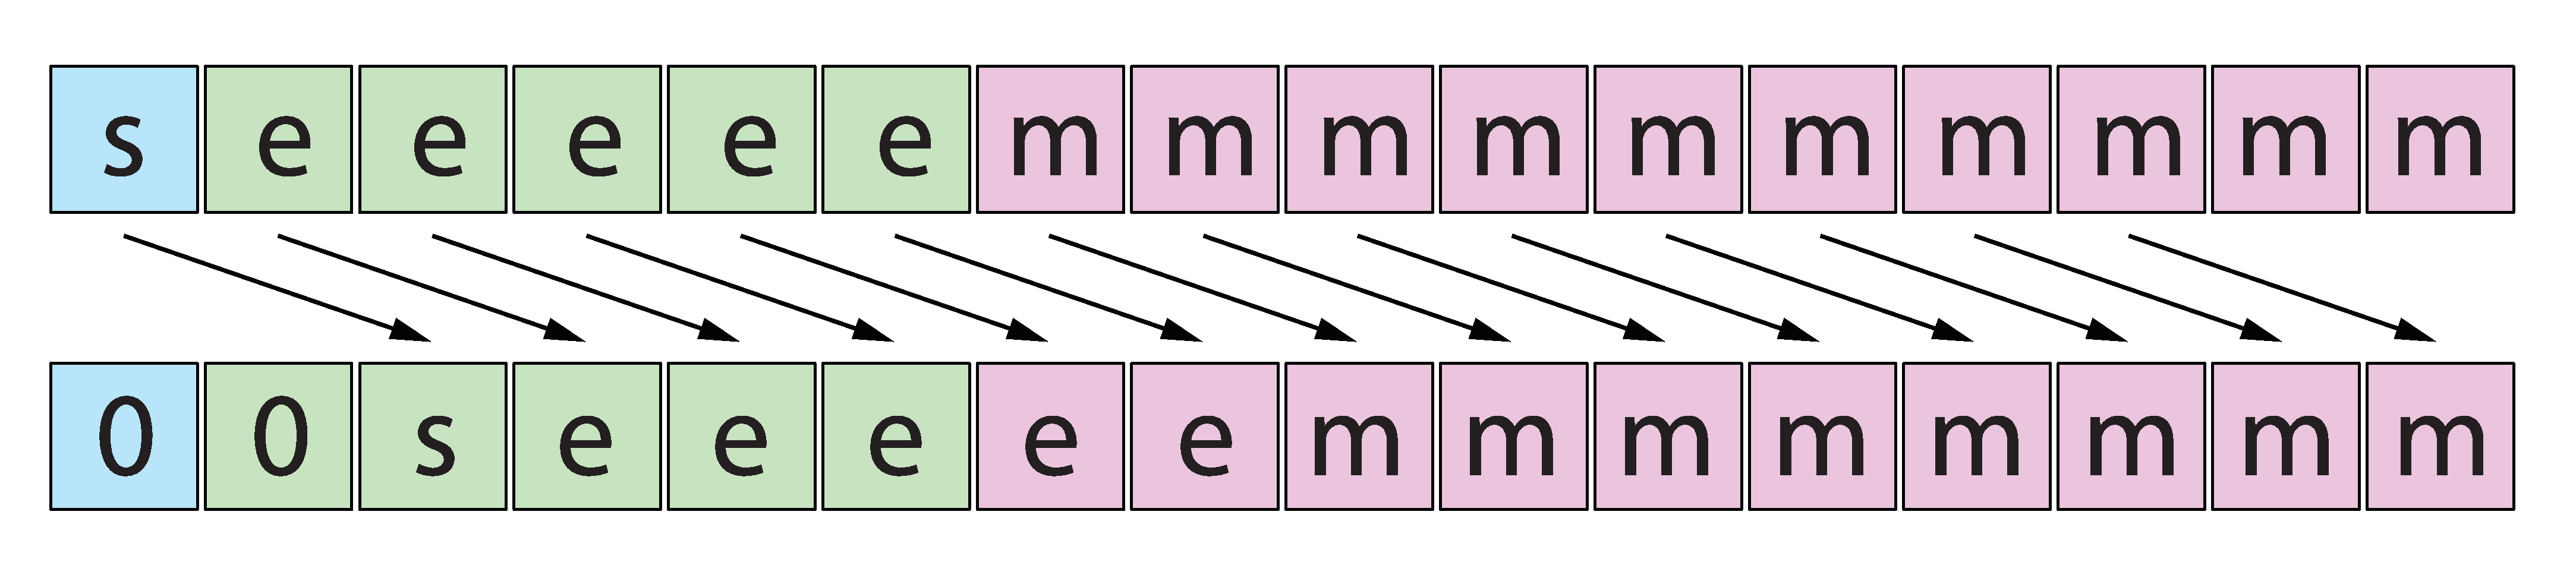
\includegraphics[width=0.9 \linewidth]{downshiftbits}

Note the different regions for sign, exponent, and mantissa.
The sign bit is shifted into the exponent, which means that the output
is always non-negative (like the rectified linear function) and is
non-linear (discontinuity at zero, as negative numbers have a much
larger exponent that positive ones). Further nonlinearity comes from
the exponential representation (shifts divide the exponent by four)
and reinterpretation of exponent bits as mantissa bits. There is
additional weirdness in the details. Shifting by two places is better
than one, as it cannot produce Inf or NaN.
% Something about its derivative?
We will also evaluate this transfer function, called \downshifttwo,
below.

I implemented all this as a modification of my custom NN training and
inference system, ``Tom7Flow.'' Tom7Flow is generally much worse than
mainstream packages; it is based on deprecated OpenCL technology, is
prone to divergence or stagnation during training due to na\"ive
choices of hyperparameters, etc. But it is at least well suited to
silly experiments that take the form, ``What if deep learning but
worse?'' such as the current exercise. In order to realize the idea
completely, I modified the inference code to calculate with
half-precision arithmetic (not just the transfer function). This means
that the trained networks can be executed using only half-precision
operations (and just addition and multiplication by constants).
Unfortunately, while my GPU supports half-precision math natively, and
OpenCL supports half-precision operations as an
extension~\cite{openclextensions}, this extension is somehow not
supported (??) by my drivers, perhaps because OpenCL is so thoroughly
deprecated. It does support half precision as a *storage* format,
which allows you to write a full-precision float to a 16-bit value
(rounding to half) or read a 16-bit half into a float (all half values
can be represented exactly in full precision). So with this one
operation it is straightforward to implement half-precision addition
and scaling. You maintain the invariant that any float value is always
exactly a half, and after you perform addition or multiplication, you
round to half (by storing in a 16-bit memory location and reading it
back). This definitionally produces the same results as the native
operation.\footnote{I also verified consistent results using the
  \verb+half.h+ software implementation. Many of the evaluation
  results quoted in the paper are actually executed on the CPU
  using this library.}

I initially tried a version of training that worked entirely using
half precision (network parameters are half, backpropagated errors and
update values are half, etc.). This worked badly. It is ideologically
unnecessary, as we just care about producing a final model that,
during inference, only executes linear half-precision operations (but
abuses floating point roundoff to do something interesting.) This
network can be trained using non-linear techniques (and must anyway,
since for example its computed derivative is not linear). So during
training, calculations are done using full-precision floats, except
for the forward step (where we round to half after every operation).
In addition to being simpler, representing intermediate learned
weights as floats seems to help training approach the final half
values smoothly, avoiding stalls due to underflow.

\subsection{Neural network experimental results}
In order to evaluate this transfer function, I ran a suite of
benchmark problems. For each problem, I compare the same network
architecture (i.e.~the number of layers, their connectivity, random
initialization, etc.) but using different transfer functions.

The transfer functions are:

\begin{itemize}
\item {\bf grad1}: The ``linear'' transfer function \gradone\ described above.
\item {\bf tanh}: The hyperbolic tangent function, which is a classic saturating (output is always in (-1, 1)) sigmoid.
\item {\bf logistic}: The function $1 / (1 + e^{-x})$, another classic sigmoid (but whose output is in (0, 1)). Each operation is performed with half precision.
\item {\bf leaky relu}: The rectified linear unit, but with a small slope below zero: \verb|x < 0.0 ? 0.1 * x : x|. This is the function I usually prefer in practice; its advantage over the standard relu is that it does not ``die'' (zero propagated error) when its input is negative.
\item {\bf downshift2}: Interpreting the half-precision input as a 16-bit word, right shift by 2 places, then reinterpret as half.
\item {\bf plus64}: $f(x) = x + 64 - 64$. This about the simplest function that has obvious rounding error. It only outputs 25 distinct values in [-1, 1] so its derivative is degenerate; I use its ``mathematical'' derivative $f'(x) = 1$.\footnote{Learning with this function might work better if we instead approximate the derivative by something non-constant, like by computing the derivative of a smoothed version. However, due to implementation tricks in Tom7Flow, we need a derivative that is expressed in terms of the transfer function's {\it output} (i.e.~$g(f(x))$ = $f'(x)$); we would not be able to express the smoothed derivative because there are only 25 distinct values of $f(x)$ in the [-1,1] range!}
\item {\bf identity}: The function $f(x) = x$. This is an important comparison because it shows us what a ``true'' linear (both mathematically and computationally) network is capable of.
\end{itemize}

TODO: Describe derivatives above?

\paragraph{Flattened models.}
For the transfer functions that are mathematically linear, we can also
compute the equivalent linear model. This just consists of a single
dense layer, using the identity transfer function, that computes the
linear function of the input. These appear in the results as ``flat''
variants.

\paragraph{MNIST.}
The first problem is the Modified National Institute of Standards and
Technology handwriting dataset (MNIST). This is a standardized dataset
of handwritten digits (0–9) as \xbyx{28}{28} greyscale images. This is chosen
partly for trollish reasons. It dates from 1998, and even at the time
of publication, accuracy with neural networks (98.4\%) and other
techniques (99.2\%) were already extremely high~\cite{lecun1998gradient}.

For this problem, I augmented the dataset by randomly offsetting the
training images by up to two pixels in any direction, and by adding
Gaussian noise. The model's input layer is just the $28 \times 28$
greyscale values, and the output is a prediction for each of the ten
digits. The models had two convolutional layers (64 \xbyx{3}{3} features,
fully overlapping + 128 \xbyx{8}{8} features, fully overlapping; then
32 \xbyx{128}{128} features + 32 \xbyx{256}{2} features with no
overlap), then two sparse layers of 1024 nodes each, then a final
dense output layer. The same initial weights and connectivity was used
for each experiment. Internal layers use the transfer function being
evaluated, but the output layer always used the identity transfer
function. This is not a good choice for this problem (softmax makes
more sense since the output is categorical) but I wanted the linear
models to be truly linear. Using the same transfer function would have
also disadvantaged functions with limited output range; \downshifttwo\
for example can technically output 1.0, but only for very large inputs
(8192.0). The final identity layer can easily scale the useful range
of the transfer function to the nominal range of the output. (This is
essential for the chess problem below, where the output instead ranges
[-1, 1].)

See the source code for various hyperparameter settings (although if
you are trying to learn good settings for hyperparameters, my code is
not the place to look). I used the ADAM weight update
trick~\cite{kingma2014adam}, which does give me much better results
than plain SGD in my experiments.

\begin{figure}[htp]
  \begin{tabular}{rcr}
{\bf transfer function} & {\bf flat} & {\bf accuracy} \\
\hline 
logistic &   & 98.20\% \\
tanh &   & 98.93\% \\
leaky-relu &   & 99.39\% \\
plus64 &   & 82.66\% \\
grad1 &   & 97.29\% \\
identity &   & 81.96\% \\
downshift2 &   & 94.45\% \\
plus64 & $\times$ & 82.01\% \\
grad1 & $\times$ & 39.19\% \\
identity & $\times$ & 81.98\% \\
\end{tabular}

  \caption{
    Results on the standardized MNIST data set. Accuracy is the
    fraction of results from the held-out test data for which the
    highest-scoring class (digit) is the correct class.
  } \label{fig:mnistresults}
\end{figure}

\begin{figure}[htp]
  \includegraphics[width=0.9 \linewidth]{mnist-bug}
  \caption{
    Bug.
  } \label{fig:mnistbug}
\end{figure}

Results for MNIST are in Figure~\ref{fig:mnistresults}.
A nice bug appears in Figure~\ref{fig:mnistbug}.

\paragraph{CIFAR-10.}
Another classic dataset comes from the Canadian Institute For Advanced
Research. They capitalize ``For'' so that the acronym can be
pronounced nicely. I mean to be fair MNIOSAT would have a certain ring
to it too. This dataset contains 60,000 RGB images of size $32 \times 32$, that
are labeled into 10 classes: Airplanes, cars, birds, cats, deer, dogs,
frogs, horses, ships, and trucks~\cite{krizhevsky2009learning}. It is
very similar to the handwriting problem but more challenging (state of
the art accuracy is more like 96.5\%). Like with MNIST, I augmented the
training set by randomly shifting the images and adding Gaussian
noise. The network structure is the same as in the MNIST problem,
except that in the first convolutional layer, each window is three
times as wide to account for the three color channels.

\begin{figure}[htp]
  \begin{tabular}{rcr}
{\bf transfer function} & {\bf flat} & {\bf accuracy} \\
\hline
sigmoid &   & 56.83\% \\
tanh &   & 67.82\% \\
leaky-relu &   & 73.11\% \\
plus64 &   & 43.60\% \\
grad1 &   & 53.56\% \\
identity &   & 41.07\% \\
downshift2 &   & 46.54\% \\
plus64 & $\times$ & 32.76\% \\
grad1 & $\times$ & 30.58\% \\
identity & $\times$ & 41.04\% \\
\end{tabular}

  \caption{
    Results on the standardized CIFAR10 data set. As with MNIST,
    accuracy is the fraction of results from the held-out test
    data for whom the highest-scoring class is the correct class.
  } \label{fig:cifar10results}
\end{figure}


Results for CIFAR-10 appear in Figure~\ref{fig:cifar10results}.
One of the nice things about using standard problems is that we
can understand how the results stack up against other researchers.
Consulting a leaderboard of public results~\cite{benenson2023are}
I see that the worst publicly known accuracy for CIFAR-10 is 75.86\%~\cite{mcdonnell2015enhanced}.
The best result for the current work, using the sensible Leaky Relu transfer function,
is 73.11\%. So this is\ldots last place. That's actually pretty good;
last place is the first winner (when counting from the end). Not to
mention that we can get into even laster place by using the other
exotic transfer functions. Even putting aside their aesthetic appeal,
I feel that these inferior transfer functions are an important
contribution to the field, as it seems to me that AI is getting too
good, and too fast! Let's take it easy there, guys!

\paragraph{Chess.}
This problem attempts to learn a good evaluation function for chess
boards. Training examples are real chess positions (from the Lichess
database) evaluated by a strong chess engine
(Stockfish~\cite{stockfish}). Stockfish generates two classes of
scores: ``Mate in N'' if one side is known to have a series of N moves
that wins (but ``Mate in 1'' is still better than ``Mate in 4''), or a
more subjective score, measured in pawns. (The score in pawns can
seemingly be higher than 64, which is kind of funny because how
are the pawns gonna fit on a 64-square board? {\large \it DUAL-WIELD?}\,\footnote{
  \begin{tabular}{p{0.35 \linewidth}p{0.50 \linewidth}}
    \chessboard[setfen=r1r1r2k/p1p1p1p1/PpPpPpPp/1P1P1P1P/BRBRBRBR/RBRBRBRB/BRBRBRBR/K1RBRBRQ w - - 0 1,tinyboard,showmover=false] &
    % this table is very confusing to tex, but fortunately we can just use
    % negative vspace! beautiful!
    \vspace{-1.05in}
  Here's an idea for a SIGBOVIK paper: What's the highest scoring chess position,
  according to Stockfish, for which it cannot deduce mate? One logistical
  challenge is that it seems to top out at +99, such as on this position
  (still no mate at depth 84).
  \end{tabular}
  })
%
Mate is of course categorically better than the pawn score, as it is
exact. Anyway, I squash this score into the range [-1, 1] and that
becomes the training instance. This network's first layer has 256
\xbyx{3}{3} convolutional features, overlapping, as well as 32
\xbyx{1}{1} and 128 \xbyx{8}{1} and \xbyx{1}{8}. Each of these is
measured in terms of squares on the board, but each square actually
corresponds to 13 inputs, for the 13 possible things that can be in
that square (exactly one set to 1.0). We also have some non-square
inputs, like the castling privileges and en passant state. So it's not
just the convolutional features but some sparse nodes too. And then we
have some more layers (you can check out the source code if you really
care about these details, which I doubt!) and then a final dense layer
with a single output using the identity transfer function as before.
No training data augmentation here, but I do normalize the board so
that it is always white to move.

For chess we can compute the accuracy, comparing to Stockfish as
ground truth (Figure~\ref{fig:chessresults}). We can also use the
evaluation function to play chess. These chess ``engines'' just look
at the possible legal moves and take the move that is most favorable,
using the learned evaluation function (no game tree search). Playing
against the best of these (``leaky'') it subjectively makes decent
moves most of the time and can even beat me playing casually. I
noticed that it had a lot of trouble ``sealing the deal'' in totally
winning positions (which is not unusual for engines that don't do
game-tree search or use endgame tables), but the problem was actually
more shallow: Due to a bug\footnote{ I used the annotations like
  \verb|[%eval #12]| that appear on moves for many games in the
  Lichess database. I didn't notice that they do not appear on a
  game-ending move like \verb+Qh4#+! This does sort of make sense
  because the eval scores would have to be \verb|[%eval #+0]| (``mate
  in 0'') or \verb|[%eval #-0]| (necessitating use of the floating
  point coprocessor) to express the winner, and there does not seem to
  be a natural way to express the definite value of stalemate. } in the
way training examples are gathered, the models were never exposed to
checkmate or stalemate positions! Since training takes several days
per function and the iron-fistedly punctilious SIGBOVIK deadlines were
imminent, there simply wasn't enough time to retrain them with access
to these positions. However, since mate is a mechanical fact of the
game (like what moves are legal) it seemed reasonable to fix this in
the engine itself: When considering all the legal moves to make, it
infinitely prefers a move that results in checkmate, and considers a
move resulting in stalemate to have score 0.0, and otherwise uses the
evaluation function. These ``fix'' versions of each engine perform
very significantly better, although they likely overestimate the
performance we'd get by actually fixing the model; there's no
guarantee that it would be able to accurately recognize mate, and the
fixed versions' greedy strategy of taking mate in 1 is always
advantageous.

These players compete against each other as well as the engines from
the Elo World project~\cite{murphy2019eloworld}, giving a sense of
their strength in an absolute scale (Figure~\ref{fig:elo}). The raw
versions perform reasonably; they all work better than a simple engine
like ``take the move that minimizes the number of moves the opponent
will have,'' (\verb+min_oppt_moves+). The fixed versions are much
better, as expected. The ``linear'' engine using the
\gradone\ transfer function, is competitive with the NES Chessmaster
engine, and outperforms a 50\% dilution of Stockfish. This is pretty
solid given that it is doing no explicit game tree search. In fact
(aside from the wrapper implementing the rules of chess and finding
the maximum eval score), it is only performing a fixed expression of
floating point addition and scaling! We could make this even more
ideologically pure using techniques from Section~\ref{sec:sixtyfive}.

\begin{figure}[htp]
  \begin{tabular}{rrr}
{\bf transfer function} & {\bf loss} & {\bf accuracy} \\
\hline 
sigmoid & 0.168 & 72.046\% \\
tanh & 0.117 & 78.527\% \\
leaky-relu & 0.118 & 78.172\% \\
plus64 & 0.162 & 75.406\% \\
grad1 & 0.111 & 78.924\% \\
identity & 0.161 & 75.975\% \\
downshift2 & 0.211 & 68.066\% \\
\end{tabular}

  \caption{
    Results of learning Stockfish's position evaluation function.
    Stockfish scores are normalized to a [-1, 1] scale, and loss
    here is the average (L1) distance between the predicted score
    and actual Stockfish score, on some 100,000 positions from
    games not in the training set. Accuracy is the percentage of
    predictions whose sign agreed with Stockfish (e.g.~they both
    agree the white player is winning).
  } \label{fig:chessresults}
\end{figure}

\begin{figure}[htp]
  % This is the output of elo.exe but I manually inverted the
  % background colors to make it print better.
  \includegraphics[width=\linewidth]{elo}
  \caption{ Results of a chess tournament. Players include ones based
    on the learned position evaluation with different transfer
    functions; these players simply take the move that results in the
    most favorable eval (no game tree search). They compete with some
    standardized players from the Elo~World
    project~\cite{murphy2019eloworld}. Rows represent the player as
    white, columns as black. A green cell means that White generally
    wins; blue a draw; red a loss. An $\times$ in a cell means that
    this outcome occurred in every game. The left column is the
    resulting Elo rating~\cite{elo1978rating}. The best model
    {\tt leaky\_fix} performs decently well, similar to NES Chessmaster
    or a Stockfish diluted to about $60\%$ strength with random
    moves (both of these engines perform game tree search). The
    centerpiece of the paper is the ``linear'' \gradone\ transfer
    function; here its learned chess player slightly outperforms
    Stockfish diluted to $50\%$ strength with random moves.
  } \label{fig:elo}
\end{figure}

\paragraph{What transfer function is best?}
The results on each of these problems are similar: The ``leaky
rectified'' transfer function is generally best or close to best.
The identity transfer function, which yields a simple linear model,
is generally worst or close to worst. The sigmoid functions are
all over the place. The experimental \downshifttwo\ function is
generally bad, perhaps because its output is strictly positive or
it has such a small dynamic range. The small amount of nonlinearity
introduced by \plussixtyfour\ does seem to give it a small edge
over the identity, but its lack of an interesting derivative and
the fact that it only produces a small number of output values seem
to be limiting. Importantly, the \gradone\ function---the
centerpiece of the first third of this paper---performs decently on
all problems. It clearly outperforms the linear models, despite
being ``linear.''

It is also interesting to compare the flattened versions of the linear
transfer functions. These are the computed (mathematically) equivalent
single-layer linear models. For \plussixtyfour\ the flattened version
is worse in all cases; the unflattened model is taking advantage of
the discretization in some way. For \gradone\ it is dramatically
worse, both because \gradone\ models are substantially using the
roundoff error and because the mathematical version of this function
($f(x) = x \times 1.036535$) is not even a good linear approximation
of the actual result (e.g. $\gradone(1) = 1$). Finally, the result
for the identity transfer function should be mathematically equivalent,
but it does not always produce the same results. This is unsurprising
since we know that floating point calculations are not perfectly
accurate, but it does hint that deep networks may make use of
floating point roundoff internally, even if they are not using silly
transfer functions!

\smallskip
Having proved the professor wrong, we could stop there, but did huge
mathematical breakthroughs ever arise from taking the option to stop
there?!


\section{Non-monotonic functions}
Because of the way that addition and scaling are defined (do the real
mathematical operation, then round), they preserve monotonicity: If $x
\geq y$, then $f(x) \geq f(y)$. But this is only true if we limit the
form of the function to a series of additions and (positive) scaling.
There are other expressions that are mathematically linear but don't
take that form; for example:

% FIXME XXX TODO

$$f(x) = x + 0.25 - x$$

This is mathematically equivalent to $f(x) = 0.25$, but with floating point, it
is a boxcar function (CHECK)

% XXX this would instead be zigzags, right?
\begin{center}
\includegraphics[width=0.75 \linewidth]{boxcar25}
\end{center}

It takes the value 0.25 in places where there is enough precision to
represent $x + 0.25$, or 0 when $x + 0.25$ rounds to $x$.

Here is $f(x) = \gradone(x) - x$, which is also linear:
\begin{center}
\includegraphics[width=0.75 \linewidth]{grad1minusx}
\end{center}

Generally speaking, we can create a large variety of functions by
computing the interference patterns between other functions, since the
sum or difference of two ``linear'' functions is also ``linear.'' In
general we'll consider expressions of this form:

\[
\begin{array}{rrl}
E & ::= & x              \\
  &  |  & E * {\tt c}    \\
  &  |  & E + {\tt c}    \\
  &  |  & E + E          \\
\end{array}
\]

Where $x$ is the function variable, and {\tt c} is one of the 63,488
finite half-precision constants. We can derive negation $(E * -1)$ and
subtraction of constants $(E + -{\tt c})$ and expressions $(E + (E *
-1))$ since every number has an exact negation by flipping its sign
bit. Exact division is possible when $\sfrac{1}{{\tt c}}$ is
representable, and there is almost always a close approximation.

This formulation leads to a tempting approach for approximating a
function iteratively, like a Taylor series. Given a target function
like $\mathrm{sin}(x)$, we can begin with an approximate expression for it,
like $x$, and then add and subtract terms to improve the
approximation. I don't know of any systematic way to improve the
approximation at each step (they are not well-behaved mathematically,
and I am not good at math), but by using computer search I can sure
make some complicated functions with many different shapes.

It is fun to watch an animation of the successively improving
approximations, but you can't see that since you're reading an
old-fashioned paper. Perhaps you can find a video of this at
\verb+tom7.org/grad+.

\subsection{Fractals} \label{sec:fractals}
Next, I endeavored to deploy these functions for something useful:
Fractals. Famously, fractals are simple functions with complex (often
literally) behavior. For example, the Mandelbrot set considers each
complex point $c$ (plotted on the plane as $x + yi$) and computes
whether $z_i$ = $z_{i-1}^2 + c$ diverges or not. It's lovely, but
squaring is not linear!

What if we just create a linear function that approximates $f(x) = x^2$?
This is definitely possible, using the approach described above. After
184 successful error-reducing rounds we get the following approximation,
with 112,204 linear operations:

\begin{center}
\includegraphics[width=0.55 \linewidth]{square}
\end{center}

Aside from the funny business near the origin, this is a fairly
accurate approximation of the square function, so you might hope that
it would draw a perverted Mandelbrot set. Unfortunately, it produces
a much sadder blotch (Figure~\ref{fig:squarebrot}). To see why, consider
the normal definition of squaring for a complex number:

\[
\begin{array}{rcl}
  (a + b\mathrm{i})^2 & = & a^2 + 2ab\mathrm{i} + b^2\mathrm{i}^2 \\
                      & = & a^2 + 2ab\mathrm{i} - b^2 \\
\end{array}
\]

Note that the real coefficient $a$ ends up part of the imaginary
coefficient $2ab$ in the result, and the imaginary coefficient $b$
becomes part of the real part (because $\mathrm{i}^2$ is real). This
means that squaring a complex number cross-pollinates between the two
components, yielding a kind of wacky rotation if we think of them as
2D coordinates.

But here, squaring is approximated as a series of operations
of the form $w_1 + w_2$ and $w \times c$ for constants $c$.
These operations on complex numbers are less interesting:

\[
\begin{array}{rcl}
  (a_1 + b_1\mathrm{i}) + (a_2 + b_2\mathrm{i}) & = & (a_1 + a_2) + (b_1 + b_2)\mathrm{i} \\[1em]
  (a + b\mathrm{i}) \times c & = & ac + bc\mathrm{i} \\
\end{array}
\]

Alas, these operations are boring; the real parts always stay real and
the imaginary parts always stay imaginary. This is why the crummy
blotch has all sorts of vertical and horizontal lines in it: As we
iterate the function we are iterating two independent components, and
the resulting picture is just some interference pattern between them.

This seems pretty definitive. Even if we had some kind of hardware
implementation of complex numbers with rounding error to abuse, there
would be no reason to have the linear operations do any
cross-pollinated rounding. Professors take note: The complex numbers
do provide some refuge!

\begin{figure}[htp]
  \includegraphics[width=0.95 \linewidth]{squarebrot}
  \caption{
    A garbage ``fractal'' that results from trying to approximate
    squaring of complex numbers using linear complex operations. Alas, it
    cannot be done. The complex numbers are truly special.
  } \label{fig:squarebrot}
\end{figure}

Still, a lot of chaos can emerge from these functions that should not
be possible with ``linear'' ones. For example, here is a complicated
function made by stringing 36,637 addition and scaling operations
together:

\begin{center}
\includegraphics[width=0.75 \linewidth]{perm16good2}
\end{center}

\begin{figure}[htp]
  \includegraphics[width=0.95 \linewidth]{perm16frac}
  \caption{
    A fractal made from iterating a ``linear'' function $f$. The color
    is the magnitude of $z_{256}$ with $z_i = f(z_{i-1}) \times c$.
    $c$ is the complex coordinate $x + y\mathrm{i}$, a constant.
  } \label{fig:perm16frac}
\end{figure}

Iterating this function produces chaotic results because of its
nonmonotonicity. In Figure~\ref{fig:perm16frac} I plot (using color)
the magnitude of $z$ after 256 iterations of

$$z_i = f(z_{i-1}) \times c$$

This is mathematically linear (as $c$ is a constant and $f$ a linear
function). Nonetheless, it produces an appealing picture. I think this
is a fractal in the sense that it is chaotic, has a color gradient,
and could be on the cover of an electronic music album. It is not a
fractal in the sense that if you zoom in on it, you get infinite
detail of self-similar shapes. In fact, if you zoom in on it only a
modest amount, you encounter rectangular pixels as you reach the
limits of half-precision floating point. (And because this fractal is
built by abusing those very limits, it is not even possible to get
more detail by increasing the accuracy!)
% what does it look like if rendered with floats instead?


\subsection{Bonus digression: Baffling numbers}
Imagine you are my professor. You assign a class project to ``make
fractals using floating point roundoff error,'' for some reason. You
spot me in the computer lab and I'm obviously way off track, because
on-screen is some kind of {\Large \it 3D fractal}. The Mandelbrot set cannot
be extended to three dimensions, you say, because of the Frobenius
theorem: Only algebras of dimension 1 (real numbers), 2 (complex
numbers) and 4 (quaternions) work~\cite{frobenius1878lineare}. Unclear
how the professor speaks the citation aloud in this scenario. I say I
``know'' this fact, but I ``don't care.'' You say that my
three-dimensional algebra can't be associative, because that's ``just
a mathematical fact.'' I say you know what else isn't associative?
{\em The floating point numbers, my dude}.

Enter the {\bf baffling numbers}, ill-advised extensions of the
complex numbers to three dimensions. Here we have numbers of the form
$a + b\mathrm{i} + c\mathrm{j}$. Addition is just pointwise, and there
are several options to complete the story for multiplication, namely
the values of the cells $A$, $B$, and $C$ in this table:
%
\[
\begin{array}{c|ccc}
  \multicolumn{1}{c}{\times} & 1          &  \mathrm{i} & \mathrm{j} \\
  \cline{2-4}
  1          & 1          &  \mathrm{i} & \mathrm{j} \\
  \mathrm{i} & \mathrm{i} & -1          & U \\
  \mathrm{j} & \mathrm{j} &  V          & W \\
\end{array}
\]

% What I actually used:

% AR, AI, AJ,
% BR, BI, BJ,
% CR, CI, CJ

% 0, 1, 0,   = i
% 0, 0, 1,   = j
% 1, 0, 0    = 1

The cells $U$, $V$, and $W$ are baffling numbers (i.e.~each some
$a + b\mathrm{i} + c\mathrm{j}$). Some choices are
degenerate, but this gives us a family of options. It is known that no
matter the choices, this does ``not work'' (in the sense that the
resulting algebra is not associative\footnote{Or else is equivalent to
  the complex numbers.}) but we don't need associativity to draw
fractals. Plus, who's gonna stop me, FROBENIUS??

\begin{figure}[htp]
  \includegraphics[width=0.95 \linewidth]{bafflebrot}
  \caption{
    The 3D ``bafflebrot'' sliced in half and projected to 2D.
    This fractal was created with the ``illegal'' number system
    called the {\it baffling numbers}. They're like the complex
    numbers but more so. The object is truncated along its
    $\textrm{j}$ axis, showing a perfect ripe Mandelbrot inside.
  } \label{fig:bafflebrot}
\end{figure}

I tried a few options, but thought that $U = \textrm{i}$, $V =
\textrm{j}$ and $W = 1$ produced satisfyingly trippy results. The
Mandelbrot is straightforwardly generalized to the ``Bafflebrot'' (the
starting point $c$ is just a baffling number now; everything else is
the same). I generated a 3D object by defining an implicit surface
based on whether a sampled point is still inside the set after 25
iterations, using Marching Cubes~\cite{lorensen1987marching} to
discretize it. The resulting mesh is 2 gigabytes and crashes every
library that attempts to programmatically simplify it. I do admire and
encourage its defiant spirit. A rendering appears in
Figure~\ref{fig:bafflebrot}.

\medskip
Drawing fractals is fun and everything, but I grew weary of the
exercise because there is no real goal other than to make a cool
picture. Instead I turned to something with a clearer challenge to
overcome: Linear Cryptography.

\section{Linear cryptography} \label{sec:eightbitchoppy}
Cryptography is like fractals minus drugs. One of the most basic
components of cryptography is a pseudorandom number generator. This
kind of function takes some state and produces a new state that
``looks random.'' Given a pseudorandom number generator, we can
construct one-way functions (``hash functions'') and from those we can
make symmetric ciphers (using, say, a Feistel network), with which we
can encrypt and decrypt data.

Another thing that professors will tell you about cryptography is that
good cryptographic functions cannot be linear. In this context, linear
includes in a finite ring like $\mathbb{Z}_{256}$ or (especially)
$\mathbb{Z}_{2}$, i.e.~bits.\footnote{So XOR is considered linear
  here, even though we previously observed that there is no linear
  function on real numbers that fits it!} One good reason for this is
that even if the function is {\em a little bit linear} then linear
cryptanalysis can be used to recover bits of the key with a lot of
example data~\cite{matsui1994linear}. Standard advice is to alternate
both linear (e.g.~XOR, or multiplication mod $2^n$) and non-linear
(e.g.~substitution) operations. (``[Substitutions] are generally the
only nonlinear step in an algorithm; they are what give a block cipher
its security.''\footnote{{\it Applied Cryptography}, Second Edition,
  page~349~\cite{schneier1996applied}.}) Of course we will prove this
adage wrong by developing a good pseudorandom function that uses only
``linear'' operations on half-precision floating point numbers.

% Here's a good readable description of linear cryptanalysis of DES:
% https://www.apprendre-en-ligne.net/crypto/bibliotheque/PDF/lincrypt.pdf

In terms of goals, pseudorandom number generation has a more clear
objective than fractals, although it's not so easy to pin down
formally. We don't even know if such functions exist,
mathematically~\cite{haastad1999pseudorandom}, although there are
generators that are provably secure assuming some other problems are
actually hard~\cite{blum1986simple} (but these problems are only {\em
  believed} to be hard). There exist many functions that look like
good pseudorandom generators, but that actually have back doors that
make them easy to predict. (Iteration of a symmetric encryption
algorithm like AES, with the key hidden, has this
property.)\footnote{And let us never forget that RSA DSI (yes, that
  RSA) took a \$10 million bribe from the NSA to put a backdoor in one
  of their pseudorandom number generators~\cite{reuters2013secret}!}
Practically speaking, though, we can subject the function to a wide
variety of statistical tests, and if it looks random to every test,
then this gives us good confidence.\footnote{Truly good cryptographic
  algorithms are also openly studied by experts. Of course nothing in
  here is to be used seriously, and not just because these algorithms
  are ridiculously slow. But I guess if you are stuck on a desert
  island with only the floating point addition and scaling operations,
  and a copy of this paper, then it would be a reasonable starting
  point for encrypting your messages. I do not recommend, if stranded
  on a desert island, to send encrypted messages: They may not be
  readable to your potential rescuers!}

Specifically, my goal is to design an algorithm that takes 64 bits of
data (represented as half-precision floats) to another 64 bits, such
that the stream of low-order bits from iterating this function passes
the TestU01's ``Big Crush'' suite of 106 statistical
tests~\cite{lecuyer2007testu01}. This suite is a successor to
Marsaglia's ``DieHard'' battery of tests~\cite{marsaglia1996diehard},
itself an improvement on Knuth's tests from The Art Of Computer
Programming~\cite{knuth1997art}.

The basis of this function is the classic substitution-permutation
network. First, each of the eight bytes are substituted with a
different byte using a table (this is the mathematically non-linear
step). Then, the 64 bits are permuted. Finally, some of the bytes are
modified additively. An illustration appears in Figure~\ref{fig:cipher}.

\begin{figure}
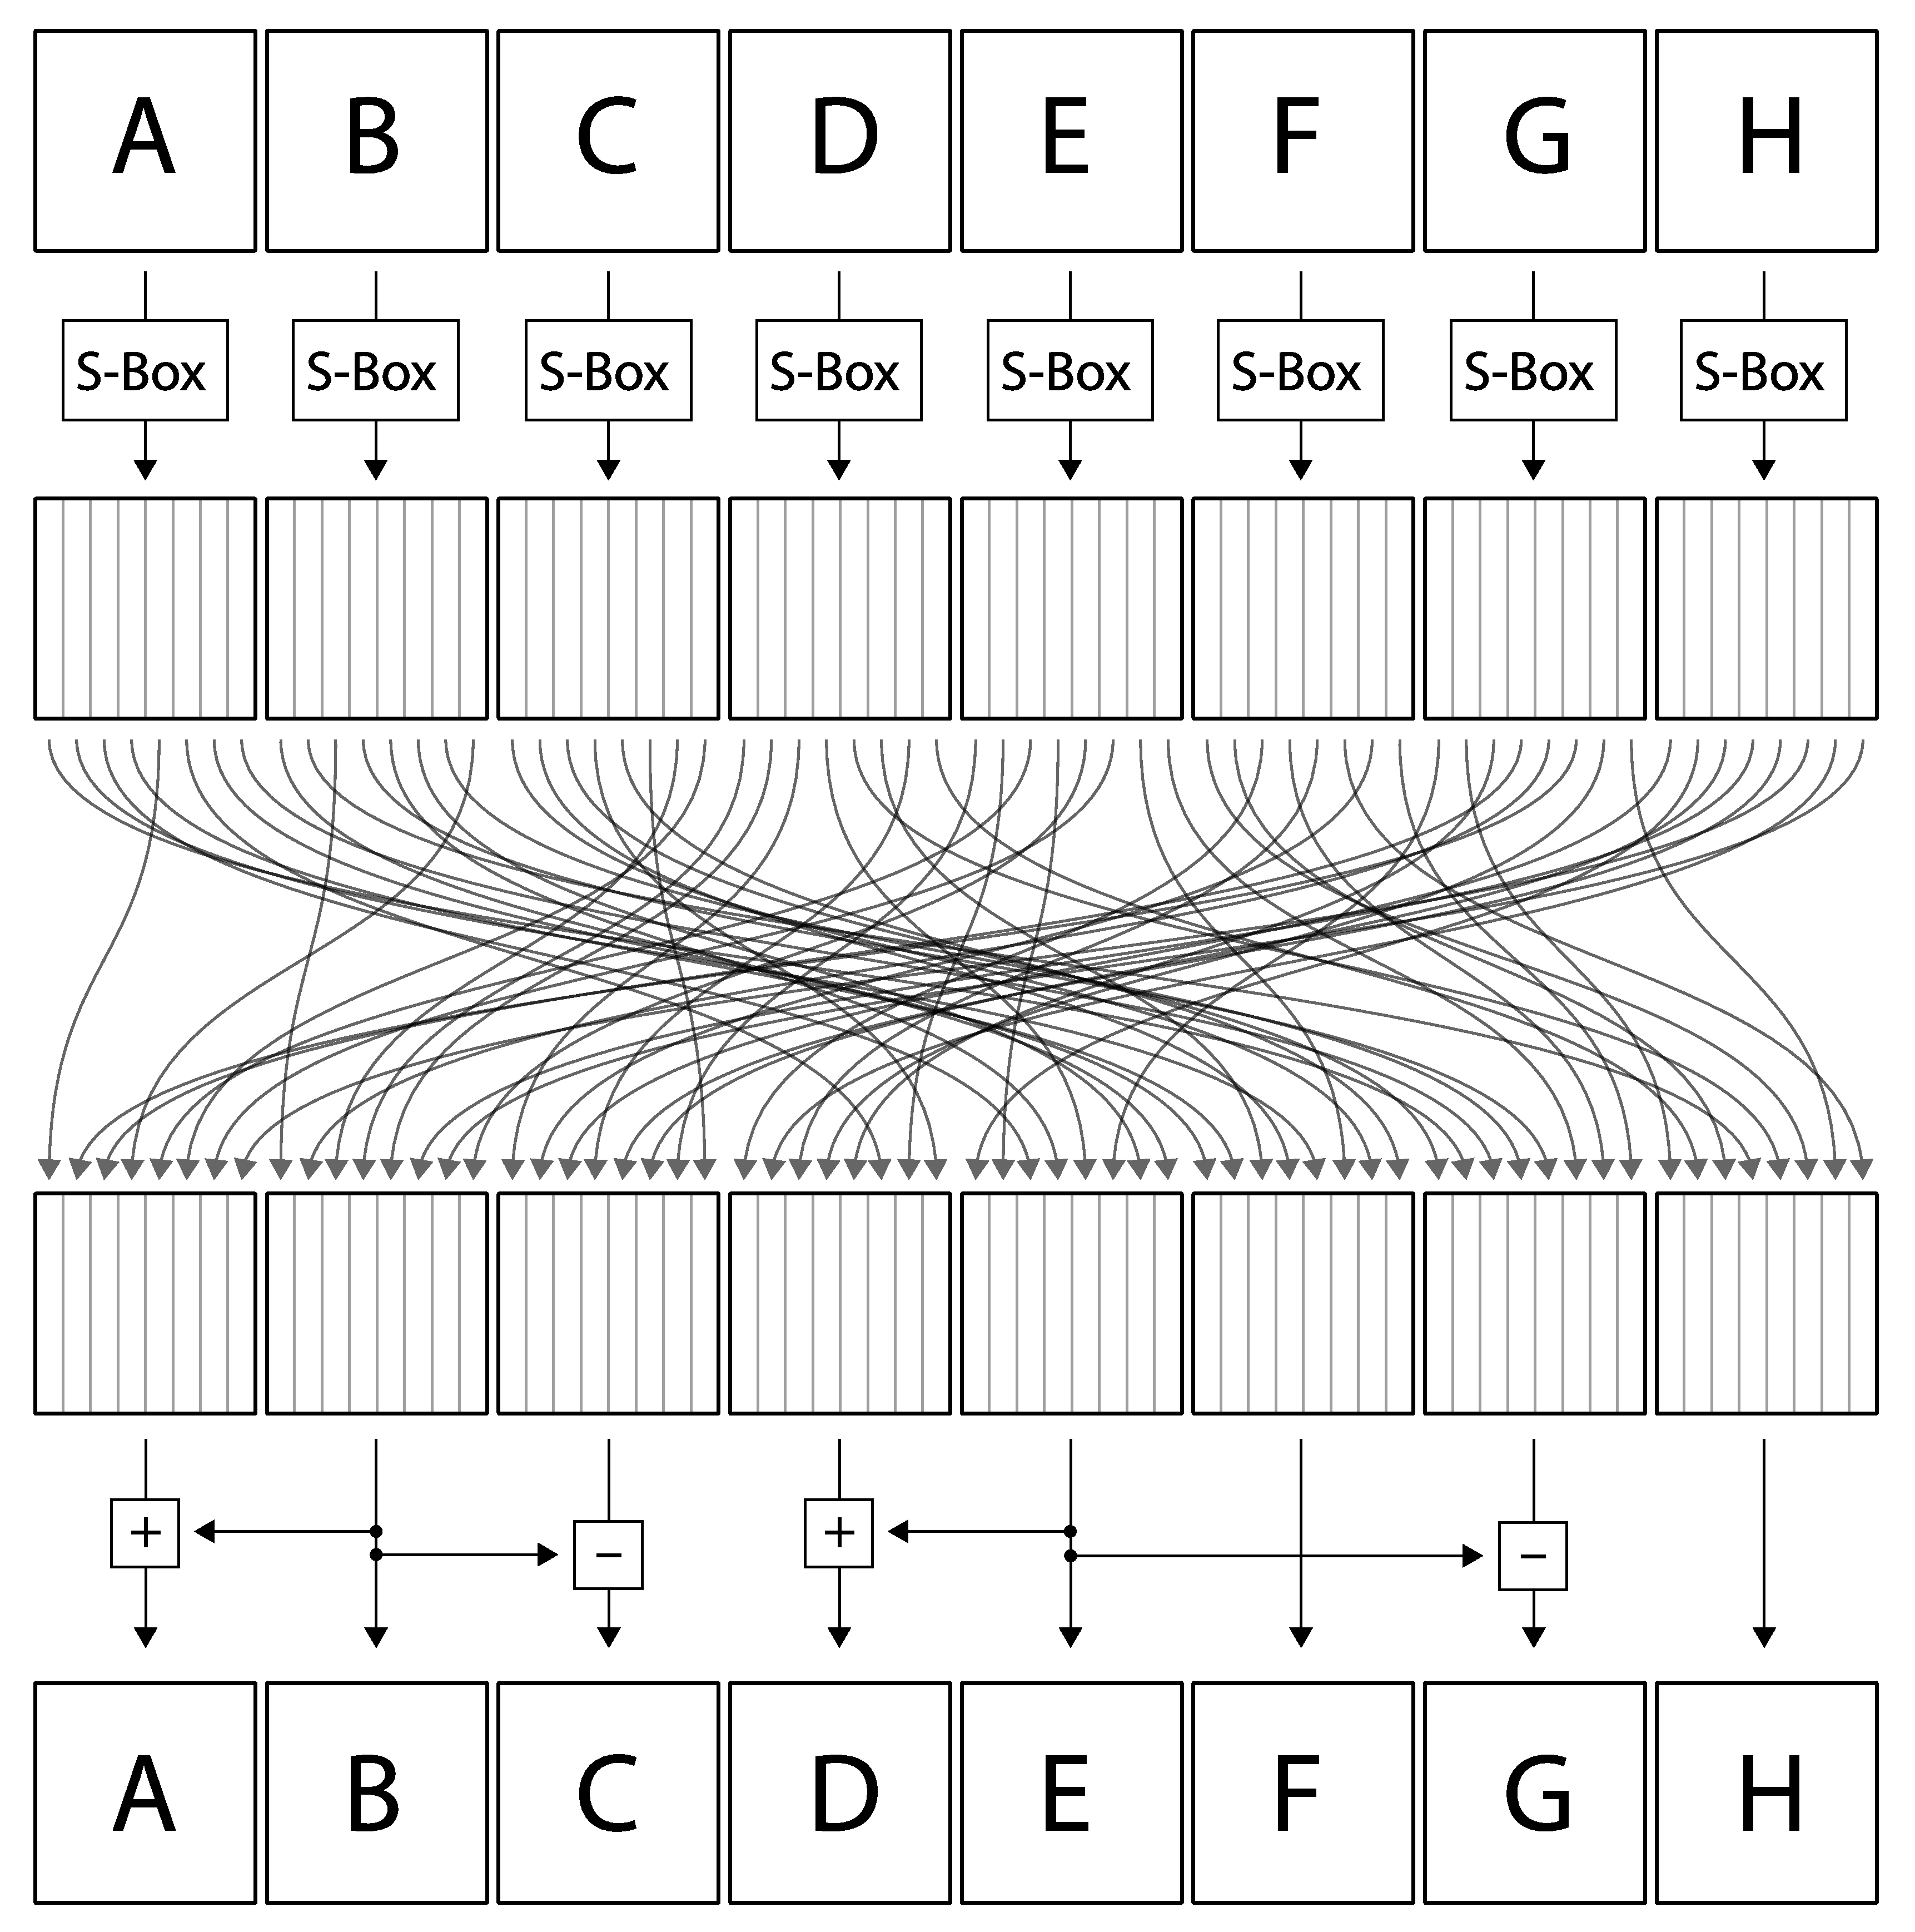
\includegraphics[width=\linewidth]{cipher}
\caption{The substitution-permutation network that forms a half decent
  pseudorandom number generator. The same substitution (``s-box'') is
  applied to each byte. Then the 64 bits are permuted. Finally, bytes
  are combined with modular addition and subtraction. This function
  passes the ``Big Crush'' suite and can be implemented with only
  half-precision floating point addition and scaling.
} \label{fig:cipher}
\end{figure}

The substitution table (``s-boxes'') was generated by computer search
with an objective to maximize the ``avalanche property'' (when a bit
of the input is complemented, about half of the output bits should be
complemented). The permutation was generated to maximize dispersion;
each quartet sends each bit to a distinct quartet in the output. This
is not the important part. We could have just used known good tables.

To implement this with half-precision floating point, we could
represent each bit with its own half, but that is no fun. The state
will be represented with eight half-precision floats, each
representing one byte's worth of information. A byte will be stored as
a values in [-1, 1), with each $\sfrac{1}{128}$ interval representing
one of the 256 values (0 is anything in [-1, -0.9921875), 1 is
anything in [-0.9921875, -0.984375), and so on). This means that
iterating the function on {\em any starting value} in the [-1, 1]
interval will produce pseudorandom results. So for example
we can guarantee that a ``fractal'' plotted using this function
will look ``fully messed up'' and not just have a few
distinguished points of randomness.
% (redundant with below.)
% \!\footnote{In fact the chaotic
%  function used to make fractals in Section~\ref{sec:fractals} was
%  an early attempt to create a 4-bit permutation using the
%  iterative approximation approach. Although it gets reasonably
%  close to the goal, it does not work for cryptography because
%  iterating it tends to reach fixed points or short cycles.}
I'll say now that this is unnecessarily hard; in the next
section of this paper we'll see a vastly more efficient
approach for handling discrete data. But working on the entire domain
makes for some challenging problems and shows that we've developed
substantial mastery of the continuous case.

Speaking of which, my first approach was to try to approximate the
substitution function (since it replaces one 8-bit byte with another,
it corresponds to a single discontinuous function of type $half
\rightarrow half$) using the iterative approach described in
Section~\ref{sec:fractals}. Although it is possible to get reasonable
approximations with this method (most values are transformed to a
value near the desired one), this will not suffice; when iterating the
function we find that the value easily gets stuck in short cycles due
to this inaccuracy.

I found a better approach, by creating a composable family of functions
that isolate specific intervals of interest. For example,

% 0 0 0 0 0 0 0 0 0 0 0 0 0 0 0 0 0 0 0 0 0 0 0 0 0 0 0 0 0 0 0 0 0 0 0 0 0 0 0 0 0 0 0 0 0 0 0 0 0 0 0 0 0 0 0 0 0 0 0 0 0 0 0 0 0 0 0 0 0 0 0 0 0 0 0 0 0 0 0 0 0 0 0 0 0 0 0 0 0 0 0 0 0 0 0 0 0 0 0 0 0 0 0 0 0 0 0 0 0 0 0 0 0 0 0 0 0 0 0 0 0 0 0 0 0 0 0 0 0 0 0 0 0 0 0 0 0 0 0 0 0 0 0 0 0 0 0 0 0 0 0 0 0 0 0 0 0 0 0 0 0 0 0 0 0 0 0 0 0 0 0 0 0 0 0 0 0 0 0 0 0 0 0 0 0 0 0 0 0 0 0 0 0 0 0 0 0 0 0 0 0 0 0 0 0 0 0 0 0 0 0 0 0 0 0 0 0 0 0 0 0 0 0 0 0 0 0 0 0 0 0 0 0 0 0 0 0 0 0 0 0 0 0 0 0 0 0 0 0 1 0 0 0 0 0 0
\includegraphics[width=0.95 \linewidth]{basisvec}

% XXX just fix it
% (This function is actually discontinuous.)

Within the interval [-1, 1), this function takes on exactly two
  values: zero\footnote{Actually, $-0$!} and $\sfrac{1}{128}$. It returns
  $\sfrac{1}{128}$ only for exactly the interval $[\sfrac{121}{128},
    \sfrac{122}{128})$. This is the interval that represents the
  number 249 ($128 + 121$; remember that the first 128 integers are in
  $[-1, 0)$). The expression that computes this is

\[
\begin{array}{l}
  f(x) = \\[0.5em]
  \left(
  \begin{array}{l}
    (x - \frac{9}{64} - \frac{1}{4} \times{} \frac{-1}{512} - \frac{1255}{512} \times^{\scriptscriptstyle 164} \frac{1027}{1024})\, + \\[0.5em]
    (x - \frac{1}{4} \times{} \frac{-1}{512} - \frac{597}{512} \times^{\scriptscriptstyle 188} \frac{1277}{2048} \times{} -\!1)\, + \\[0.5em]
    \frac{517}{128} \times{} -32 \\[0.5em]
  \end{array}
  \right) + \\[2em]
%
  \left(
  \begin{array}{l}
    (x - \frac{17}{128} - \frac{1}{4} \times{} \frac{-1}{512} - \frac{1255}{512} \times^{\scriptscriptstyle 164} \frac{1027}{1024})\, + \\[0.5em]
    (x - \frac{1}{4} \times{} \frac{-1}{512} - \frac{597}{512} \times^{\scriptscriptstyle 188} \frac{1277}{2048} \times{} -\!1)\, + \\[0.5em]
    \frac{517}{128} \times{} 32
  \end{array}
  \right) \times{} \frac{-1}{32} \\
\end{array}
\]

\noindent where $E \times^{n} c$ means $E \times c \times c \times c \ldots$ for $n$ iterations.
Mathematically this is equivalent to this constant function (all $x$s cancel out):
$$f(x) = \frac{13^{164} \times{} 79^{164}}{2^{1656}}$$

I spent a long time writing code to simplify these expressions and
generate \LaTeX\ for them, by the way! As usual, I thought it would
look cool when I got it working, but it just looks like a bunch of numbers.

We can think of this function as a basis vector, representing the 256-dimension
vector $\langle 0, 0, 0, \ldots, 0, 1, 0, 0, 0, 0, 0, 0 \rangle$. We'll call
this one $\basis_{249}$ since it selects the integer 249. If we can find $\basis_n$
for each $n \in \mathbb{Z}_{256}$, then we will be able to combine them
to systematically construct functions.

The one just pictured is one of the smallest expressions; most are
much larger. I wish I could tell you that I figured out the principles
underlying how to analytically generate these functions, but I
discovered them with computer search and some elbow grease.

\paragraph{Choppy functions.}
I call a function $f$ ``choppy'' if for every half precision floating point value in
$[-1, 1)$ it has the following properties:

\begin{itemize}
\item For $n \in \mathbb{Z}_{256}$ and $r \in [0, 1)$,
  $f(-1 + \sfrac{n + r}{128}) = v$ for the same value $v$. We only need to
  consider cases where $n + r$ is representable as a half.
\item $v$ is itself of the form $\sfrac{n - 128}{128}$ for some $n \in \mathbb{Z}_{256}$.
\item For these purposes, we treat the single value $-0$ as being equal to $0$.
\item And, as usual, the function is built only with floating point addition
  and scaling by constants.
\end{itemize}

That is, the function produces the same result for any representation
of an integer, and that result is the smallest representation of an
integer. These functions are maximally useful in that they are
``liberal in what they accept,'' but ``conservative in what they
return''~\cite{rfc761}. It also means that each function also can be
understood as a function $\mathbb{Z}_{256} \rightarrow
\mathbb{Z}_{256}$, so we can represent them as a vector of 256
integers. The basis vectors $\basis_n$ are those that are of the form
$\langle 0, \ldots, 1, \ldots, 0\rangle$.

I then conducted computer search for choppy functions, putting those
into a database (keyed by the corresponding integer vector). Some are
easy to find, others harder. Summing and scaling choppy functions
yield choppy functions (as long as the vectors remain integral and in
range), so I use a simplified version of Gauss-Jordan
elimination~\cite{gaussjordan} to solve for basis vectors. Once I have
$\basis_n$, this column can be changed at will for any existing choppy
function (by just adding or subtracting multiples of $\basis_n$), so
new choppy functions that only vary in that column can be ignored.

By trying a variety of operations that are known to be useful
(e.g.~iterated multiplication of constants near $1.0$) and
hill-climbing towards functions with the choppy property, it is not
too hard to find $\basis_n$ for most $n$. It seems to become more
challenging for $n$ near 128; this is the point $0.0$ in
half-precision. Specifically, the hardest problem was to make a
function that produced different results for inputs $< 0.0$ versus
inputs $\geq 0.0$. This is the {\em zero-threshold problem}.

% XXX something about optimization, which I wasted loads of time on?

\paragraph{Why is this hard?}
Distinguishing between negative and non-negative numbers is
deceptively difficult. Looking back to the function $f(x) = x + 128.0
- 128.0$ (Section~\ref{sec:plus128}), it has useful discontinuous
steps, but note that the discontinuity does not happen at zero. This
is because we are rounding to the nearest value, and so small negative
numbers near zero end up rounding to the same result that zero does.
Moreover, the resolution of the floating point numbers is highest near
zero (especially because of subnormal numbers), which exacerbates our
attempts to control rounding of them. For example, you might think
that we could simply shift this function left and right by
substituting $x + c$ for $x$ in its body. This would work
mathematically, but it does {\em not} work for floating point numbers,
because each operation performs some rounding. If this rounding ever
ends up conflating a negative number with a non-negative one, we will
not be able to recover.
% (But zero-threshold does start with adding. Why does it work?)

I found a zero-threshold function using a combination of manual and
computer search. This was some ordeal, and the resulting enormous
function is in Figure~\ref{fig:zerothreshold}. Perhaps you are
smarter than me and can find a better one!

\begin{figure*}[tp]
$zt(x) = x + \frac{1}{2^{24}} \times^{\scriptscriptstyle 9743} \frac{1025}{1024} \times{} \frac{39}{2^{19}} + \frac{1279}{16384} \times{} 4100 + 318 \times{} 4 + 1 \times^{\scriptscriptstyle 559} \frac{1025}{1024} \times{} \frac{1027}{2048} \times^{\scriptscriptstyle 1160} \frac{1025}{1024} \times{} \frac{545}{2048} \times^{\scriptscriptstyle 23} \frac{1025}{1024} \times{} \frac{311}{512} \times^{\scriptscriptstyle 137} \frac{1025}{1024} \times{} \frac{527}{2048} \times^{\scriptscriptstyle 365} \frac{1025}{1024} \times{} \frac{627}{1024} \times^{\scriptscriptstyle 346} \frac{1025}{1024} \times{} \frac{593}{1024} \times^{\scriptscriptstyle 676} \frac{1025}{1024} \times{} \frac{281}{512} \times^{\scriptscriptstyle 557} \frac{1025}{1024} \times{} \frac{129}{256} \times^{\scriptscriptstyle 830} \frac{1025}{1024} \times{} \frac{589}{4096} \times^{\scriptscriptstyle 336} \frac{1025}{1024} \times{} \frac{1029}{2048} \times^{\scriptscriptstyle 663} \frac{1025}{1024} \times{} \frac{1041}{2^{18}} - 2206 + 2206 \times{} \frac{9}{256} + 1076 + 2534 - 2074 \times{} \frac{17}{64} - 2048 + 2048 \times{} \frac{1}{8} $ \\

\scalebox{2}{$$=$$}
\[
\begin{array}{l}
\frac{593 \times{} 2187 \times{} 5^{30793} \times{} 343 \times{} 11 \times{} 169 \times{} 289 \times{} 361 \times{} 961 \times{} 41^{15396} \times{} 43 \times{} 79 \times{} 109 \times{} 281 \times{} 311 \times{} 347}{2^{154102}}\scalebox{2}{$\,x\,+$} \\[1em]
\frac{\begin{array}{r@{}l}
% XXX: Maybe could fit more of it with a small font?
\, & 84107227537103367748705454682078539303191039250504832410385579895977259206417678 \\
\, & 54245560547677512932803511681703341508665266147325419821191498222214690318490003 \\
\, & 88110778422408950986678118366271064412982414738166383752334216371785576710459496 \\
\, & 25738831829937485787963475192987844674323695457715738688221958462470493961327089 \\
\, & 64862528034085403084792949523917534005532171250047637347672007635216035917044700 \\
\, & \ldots 569\ \mathrm{lines} \ldots \\
\, & 73014930689000221762919045089322540125964944324282583780813532524840229888776299 \\
\, & 45268638388603643723804098205965854510116202420980541689175292145265852612920173 \\
\, & 68725838005728517370192463512280524432138902703991548800398876262333592383735651 \\
\, & 92764023532792804235216160403774463302046032255421688296905932246680375562746379 \\
\, & 76285400623707503241570527062342946483273904883074176883724035214883942317941586 \\
\, & 85212883934224294828781615577153021816836375301250331354703790141535016001286984 \\
\, & 69246587905140878604602957637178398679300714629238352320436905873649993209 \times{} 3 \times{} 17 \times{} 421 \\
\end{array}}{2^{154126}} \\
\end{array}
\]
\caption{
  A zero-threshold function. Returns $\sfrac{1}{128}$ for values in $[0, 1)$ (and $-0$) and $0$ for values in $[-1, 0)$.
      Top is the series of additions and scalings to perform, all from left to right. At bottom
      is the equivalent mathematical expression, but the enormous numerator cannot be printed due to
      extremely oppressive SIGBOVIK page limitations.
  } \label{fig:zerothreshold}
\end{figure*}

\paragraph{Substituting and permuting.}
In any case, with this function it was possible to form a complete basis. This basis
makes it ``easy'' to perform operations on half values that represent bytes. For
example, the s-box step substitutes some distinct byte for each different input
byte. This would normally be implemented with a table lookup. If we compute
$\basis_n(x) \times \mathrm{subst}[n]$, this returns the correct\footnote{Technically
  we need to do some multiplicative adjustments to put the value in $[-1, 1)$.}
result $\mathrm{subst}[n]$ if the input $x = n$, and $0$ otherwise.
So if we just sum all 256 of these up, exactly one of them will be nonzero,
and the correct substituted value.

Permutation is defined on the component bits. Here, we compose a function that
computes each of the eight output bytes. We use the same approach of summing
a bunch of $\basis_n(x)$ evaluations (each multiplied by the correct answer).
Here we are testing whether the input has some particular bit set (a sum of the
128 $\basis_n(x)$ functions where $n$ has that bit set), and the output is the
power of two that sets the appropriate output bit. Many of these functions would
have simpler implementations (for example, ``is the high-order bit set?'' is the
same as the zero-threshold function) but at this point I was happy to just have
something working, and taking some joy in how absurdly large the functions
were getting.

\label{sec:cryptmodularaddition}
The cipher also includes addition and subtraction mod 256. Addition
and subtraction are already available for half-precision floats, and
they have faithful behavior, so we just need to implement the wrapping-around
behavior so that the result is strictly in $[-1, 1]$.
This is straightforward with the zero threshold function;\footnote{Compare to
  the remarks ``why is this hard?'' above. Here, $zt(x - 1)$ {\em does} do what you'd want,
  shifting the threshold value from $0$ to $1$. This is because there is {\em more}
  precision near zero than near one.}
we produce a corrective factor if the result is $\geq 1$ or $< -1$ (and zero otherwise).
We then add those corrective factors produce the remainder we desire.

\comment{
\subsection{Bonus digression: Floating point horrors}

Floating point is like JavaScript. Even when you think you are approaching
some level of expertise, every time you get seriously into it, you will discover
some horror that you had never known before.

Testing the functions in this section, like the basis functions,
requires looping over the entire domain of a half-open interval like
$[-1, -1 + \sfrac{1}{128})$. We want to check that the function
  produces the same result for any of these representations of the
  corresponding integer. This is a little tricky for floating point
  numbers; we can't just ``add one'' to get to the next number,
  and the distance between representable numbers changes depending
  on where we are on the number line.

Now, I hear you say, floating point has a solution: {\tt nextafter}.
${\tt nextafter}(f, d)$, you remember, gives the next distinct
value after $f$ when moving toward the float $d$ (for example +Inf).
So we can just do a loop like

\begin{lstlisting}
for (half h = -1.0 + n/128.0;
     h < -1.0 + (n + 1)/128.0;
     h = nextafter(h, 1.0/0.0)) {
  // ...
}
\end{lstlisting}

{\large HA!} This does not work. For reasons I cannot understand,
{\tt nextafter} has a mandate special case that ``if [...] the
result is subnormal or zero, raises \verb+FE_INEXACT+ and \verb+FE_UNDERFLOW+'',
which means that {\tt nextafter} cannot be used to enumerate an interval that
contains zero, or even one that contains valid small floating point
numbers (subnormals). What? Why?
Instead, I implemented my own version that works on the binary
representation; this is slightly annoying because the negative
numbers come in the opposite order of the positive, and they
are not adjacent. But it is not as annoying as raising an
exception!

(Actually, it looks like I was just wrong about this! It does raise
exceptions but they are silent, so looping does work. I think what
was going wrong was a classic mistake: I was calling the wrong version
of nextafter (e.g. the float one), which will not work because the deltas
are too small. I think this is is because of good ol' C++ argument dependent
lookup. std::nextafter doesn't call the one from half.h, but using namespace std; nextafter
does. Cool)
}

\subsection{Benchmark results}
To evaluate the quality of the pseudorandom number generator, I used
the TestU01 ``Big Crush'' suite. This test needs a sample of 1.64
billion bits, so I actually evaluated it on equivalent code that
performs the steps using normal integer operations. Even then, the
suite takes several days to run, so I modified it to run tests in
parallel and cache the results of completed tests. This saved me from
losing data if my computer crashed or needed to be rebooted.

Results appear in Figure~\ref{fig:testu01}. Passing these tests does
not ensure that the pseudorandom number generator is good for
cryptography, although it is a good start.

\begin{figure*}[tp]
  \footnotesize
  \begin{tabular}{rl|rl|rl}
    {\bf Test} & {\bf p-value} &
    {\bf Test} & {\bf p-value} &
    {\bf Test} & {\bf p-value} \\
    SerialOver, r = 0 & $0.9653$ \\
SerialOver, r = 22 & $0.7292$ \\
CollisionOver, t = 2 (0) & $0.3890$ \\
CollisionOver, t = 2 (9) & $0.6537$ \\
CollisionOver, t = 3 (0) & $0.8046$ \\
CollisionOver, t = 3 (16) & $0.9279$ \\
CollisionOver, t = 7 (0) & $0.2906$ \\
CollisionOver, t = 7 (24) & $0.0031$ \\
CollisionOver, t = 14 (0) & $0.4310$ \\
CollisionOver, t = 14 (27) & $0.5062$ \\
CollisionOver, t = 21 (0) & $0.1909$ \\
CollisionOver, t = 21 (28) & $0.2906$ \\
BirthdaySpacings, t = 2 & $0.4179$ \\
BirthdaySpacings, t = 2 (b) & $0.5749$ \\
BirthdaySpacings, t = 3 & $0.2249$ \\
BirthdaySpacings, t = 4 & $0.2230$ \\
BirthdaySpacings, t = 4 (14) & $0.2230$ \\
BirthdaySpacings, t = 4 (0) & $0.2293$ \\
BirthdaySpacings, t = 4 (16) & $0.9111$ \\
BirthdaySpacings, t = 7 (0) & $0.8077$ \\
BirthdaySpacings, t = 7 (7) & $0.4887$ \\
BirthdaySpacings, t = 8 (14) & $0.5956$ \\
BirthdaySpacings, t = 8 (22) & $0.1382$ \\
BirthdaySpacings, t = 16 (0) & $0.5266$ \\
BirthdaySpacings, t = 16 (26) & $0.6619$ \\
BirthdaySpacings, t = 13 (0) & $0.8419$ \\
BirthdaySpacings, t = 13 (5) & $0.9242$ \\
BirthdaySpacings, t = 13 (10) & $0.3125$ \\
BirthdaySpacings, t = 13 (15) & $0.4234$ \\
BirthdaySpacings, t = 13 (20) & $0.0172$ \\
BirthdaySpacings, t = 13 (26) & $0.3276$ \\
ClosePairs NP t=3 & $0.9584$ \\
ClosePairs mNP t=3 & $0.6028$ \\
ClosePairs mNP1 t=3 & $0.3668$ \\
ClosePairs mNP2 t=3 & $0.8549$ \\
ClosePairs NJumps t=3 & $0.3739$ \\
ClosePairs mNP2S t=3 & $0.3813$ \\
ClosePairs NP t=5 & $0.2328$ \\
ClosePairs mNP t=5 & $0.4011$ \\
ClosePairs mNP1 t=5 & $0.6286$ \\
ClosePairs mNP2 t=5 & $0.7635$ \\
ClosePairs NJumps t=5 & $0.7981$ \\
ClosePairs mNP2S t=5 & $0.4369$ \\
ClosePairs NP t=9 & $0.3073$ \\
ClosePairs mNP t=9 & $0.7986$ \\
ClosePairs mNP1 t=9 & $0.1934$ \\
ClosePairs mNP2 t=9 & $0.5857$ \\
ClosePairs NJumps t=9 & $0.9882$ \\
ClosePairs mNP2S t=9 & $0.0962$ \\
ClosePairs NP t=16 & $0.3787$ \\
ClosePairs mNP t=16 & $0.1983$ \\
ClosePairs mNP1 t=16 & $0.0511$ \\
ClosePairs mNP2 t=16 & $0.2874$ \\
ClosePairs NJumps t=16 & $0.9369$ \\
ClosePairs mNP2S t=16 & $0.7523$ \\
SimpPoker 0 8 & $0.9863$ \\
SimpPoker 27 8 & $0.4528$ \\
SimpPoker 0 32 & $0.8052$ \\
SimpPoker 25 32 & $0.1166$ \\
CouponCollector, r = 0 & $0.3233$ \\
CouponCollector, r = 10 & $0.7936$ \\
CouponCollector, r = 20 & $0.2870$ \\
CouponCollector, r = 27 & $0.1878$ \\
Gap 0 16 & $0.2858$ \\
Gap 25 32 & $0.6202$ \\
Gap 0 128 & $0.7462$ \\
Gap 20 1024 & $0.1068$ \\
Run 0 & $0.3096$ \\
Run 15 & $0.5308$ \\
Permutation 3 & $0.7322$ \\
Permutation 5 & $0.8632$ \\
Permutation 7 & $0.8337$ \\
Permutation 10 & $0.7557$ \\
CPerm 0 & $0.0512$ \\
CPerm 10 & $0.0116$ \\
MaxOft, t = 8 & $0.1909$ \\
MaxOft AD, t = 8 & $0.6478$ \\
MaxOft, t = 16 & $0.3601$ \\
MaxOft AD, t = 16 & $0.7570$ \\
MaxOft, t = 24 & $0.3625$ \\
MaxOft AD, t = 24 & $0.7378$ \\
MaxOft, t = 32 & $0.4541$ \\
MaxOft AD, t = 32 & $0.1967$ \\
SampleProd, t = 8 & $0.6129$ \\
SampleProd, t = 16 & $0.7735$ \\
SampleProd, t = 24 & $0.0891$ \\
SampleMean, r = 0 & $0.1115$ \\
SampleMean, r = 10 & $0.4571$ \\
SampleCorr, k = 1 & $0.0260$ \\
SampleCorr, k = 2 & $0.0146$ \\
AppearanceSpacings, r = 0 & $0.6741$ \\
AppearanceSpacings, r = 27 & $0.0951$ \\
WeightDistrib, r = 0 (0.25000) & $0.3097$ \\
WeightDistrib, r = 20 (0.25000) & $0.6266$ \\
WeightDistrib, r = 28 (0.25000) & $0.4372$ \\
WeightDistrib, r = 0 (0.06250) & $0.6148$ \\
WeightDistrib, r = 10 (0.06250) & $0.6600$ \\
WeightDistrib, r = 26 (0.06250) & $0.6532$ \\
SumCollector & $0.6092$ \\
MatrixRank, L=30, r=0 & $0.4367$ \\
MatrixRank, L=30, r=25 & $0.3045$ \\
MatrixRank, L=1000, r=0 & $0.0841$ \\
MatrixRank, L=1000, r=26 & $0.0145$ \\
MatrixRank, L=5000, r=15 & $0.2650$ \\
MatrixRank, L=5000, r=0 & $0.9631$ \\
Savir2 & $0.7317$ \\
GCD & $0.7578$ \\
RandomWalk1 H (L=50, r=0) & $0.6779$ \\
RandomWalk1 M (L=50, r=0) & $0.9338$ \\
RandomWalk1 J (L=50, r=0) & $0.3168$ \\
RandomWalk1 R (L=50, r=0) & $0.4753$ \\
RandomWalk1 C (L=50, r=0) & $0.4941$ \\
RandomWalk1 H (L=50, r=25) & $0.8645$ \\
RandomWalk1 M (L=50, r=25) & $0.6220$ \\
RandomWalk1 J (L=50, r=25) & $0.4576$ \\
RandomWalk1 R (L=50, r=25) & $0.9736$ \\
RandomWalk1 C (L=50, r=25) & $0.6768$ \\
RandomWalk1 H (L=1000, r=0) & $0.9915$ \\
RandomWalk1 M (L=1000, r=0) & $0.8194$ \\
RandomWalk1 J (L=1000, r=0) & $0.7606$ \\
RandomWalk1 R (L=1000, r=0) & $0.4983$ \\
RandomWalk1 C (L=1000, r=0) & $0.0529$ \\
RandomWalk1 H (L=1000, r=20) & $0.3353$ \\
RandomWalk1 M (L=1000, r=20) & $0.2279$ \\
RandomWalk1 J (L=1000, r=20) & $0.8593$ \\
RandomWalk1 R (L=1000, r=20) & $0.4915$ \\
RandomWalk1 C (L=1000, r=20) & $0.9640$ \\
RandomWalk1 H (L=10000, r=0) & $0.0713$ \\
RandomWalk1 M (L=10000, r=0) & $0.4753$ \\
RandomWalk1 J (L=10000, r=0) & $0.6421$ \\
RandomWalk1 R (L=10000, r=0) & $0.0469$ \\
RandomWalk1 C (L=10000, r=0) & $0.6232$ \\
RandomWalk1 H (L=10000, r=15) & $0.5739$ \\
RandomWalk1 M (L=10000, r=15) & $0.7165$ \\
RandomWalk1 J (L=10000, r=15) & $0.6868$ \\
RandomWalk1 R (L=10000, r=15) & $0.7075$ \\
RandomWalk1 C (L=10000, r=15) & $0.2100$ \\
LinearComp, r = 0 (Num) & $0.7964$ \\
LinearComp, r = 0 (Size) & $0.8628$ \\
LinearComp, r = 29 (Num) & $0.1564$ \\
LinearComp, r = 29 (Size) & $0.9696$ \\
LempelZiv, r = 0 & $0.8373$ \\
LempelZiv, r = 15 & $0.4632$ \\
Fourier3, r = 0 & $0.9159$ \\
Fourier3, r = 27 & $0.8144$ \\
LongestHeadRun (Chi), r = 0 & $0.1270$ \\
LongestHeadRun (Disc), r = 0 & $0.9025$ \\
LongestHeadRun (Chi), r = 27 & $0.7822$ \\
LongestHeadRun (Disc), r = 27 & $0.6878$ \\
PeriodsInStrings, r = 0 & $0.6300$ \\
PeriodsInStrings, r = 20 & $0.0839$ \\
HammingWeight2, r = 0 & $0.1331$ \\
HammingWeight2, r = 27 & $0.0322$ \\
HammingCorr, L = 30 & $0.5516$ \\
HammingCorr, L = 300 & $0.7373$ \\
HammingCorr, L = 1200 & $0.9393$ \\
HammingIndep, L=30, r=0 & $0.1326$ \\
HammingIndep, L=30, r=27 & $0.7257$ \\
HammingIndep, L=300, r=0 & $0.4177$ \\
HammingIndep, L=300, r=26 & $0.7630$ \\
HammingIndep, L=1200, r=0 & $0.4981$ \\
HammingIndep, L=1200, r=25 & $0.3571$ \\
Run of bits (runs), r = 0 & $0.0241$ \\
Run of bits (bits), r = 0 & $0.5718$ \\
Run of bits (runs), r = 27 & $0.0822$ \\
Run of bits (bits), r = 27 & $0.7981$ \\
AutoCorr 1 0 & $0.3058$ \\
AutoCorr 3 0 & $0.0371$ \\
AutoCorr 1 27 & $0.3292$ \\
AutoCorr 3 27 & $0.0612$ \\

  \end{tabular}
  \caption{
    Results of the TestU01 ``Big Crush'' suite on the
    pseudorandom number generator built from floating point roundoff
    error. A p-value of $< 0.001$ or $> 0.999$ is considered
    suspect by the suite, so all tests pass here.
  } \label{fig:testu01}
\end{figure*}

Running single-threaded on a 3.0 GHz Threadripper 2990WX, this
function generates 25.8 bytes of randomness per second, which is slow.
By precomputing the substitution, permutation, and zero threshold
expressions (so they can be performed by lookup into 64k-entry tables),
it generates 18,685.2 bytes per second, which is still slow.

If we were building an encryption algorithm (a symmetric block
cipher), it would be natural to use this as its ``round function.'' In
a Feistel network~\cite{feistel1973cryptography}, each input block
(128 bits) is broken into two halves; one of them is mixed with some
key bits (for example with XOR) and then passed to this function. Its
output is XORed with the other half; the two halves are swapped, and
this ``round'' is repeated many times until we believe that the data
are suitably screwed up. Decryption is the reverse. We can use
addition and subtraction mod $2^8$ to combine the data instead of XOR
(which is addition mod $2^1$), so we already have all the operations
we need to build a whole block cipher here. As Bruce Schneier
says,\footnote{{\it Applied Cryptography}, Second Edition, page 351.}
``It is easy to design a block cipher.''


\section{THE ULTIMATE THROWBACK}
Having developed a basis for extracting arbitrary bits, we can express
any function of a single variable, and we've seen how some other
functions (like addition mod $2^8$) can be done. At this point, it
seems like we probably have the building blocks to demonstrate that
addition and scaling on half-precision floats is Turing complete. I
mean, pretty much everything is Turing complete. In the past, I built
computers that were perfect and beautiful, such as a hardware
implementation of the NaNDY 1000, a computer architecture that
computes using only floating point NaN and
Infinity~\cite{murphy2019nan}. In a concession to ideological purity,
though, the NaNDY 1000 has no I/O. So it is very boring to use.

For today's investigations of the capabilities of floating point, I'll
make the opposite concession: Let's make a computer that is exciting
to use, but that makes some (reasonable) ideological concessions so that
it can do something interesting.

\subsection{Fluint8} \label{sec:fluint}

First of all, if we want to do some serious computation, 25.8 bytes
per second isn't going to cut it. To look for performance enhancing
substances, I perused the back catalog of the world's most prestigious
conference, SIGBOVIK. There in the 2018 edition, on page 125, I found
an intriguing paper, {\it The fluint8 Software Integer Library}, by
Drs.~Jim McCann and \ldots Tom Murphy VII? Wait, that's me? {\large \em I already
wrote this paper?!}

\medskip
The {\it fluint8} library represents an element of $\mathbb{Z}_{256}$
(a.k.a.~{\tt uint8}) as a 32-bit float, and provides multiplication,
addition, subtraction, negation, division, and bitwise functions and,
or, and exclusive or.

Compared to the approach discussed in Section~\ref{sec:eightbitchoppy}
using ``choppy functions,'' {\it fluint8} has much more simple and
sensible implementations of functions like addition:

\begin{lstlisting}
inline float fu8_add(float a, float b) {
  float x = a + b;
  x -= x - 127.5f + 3221225472.0f - 3221225472.0f;
  return x;
}
\end{lstlisting}

The \verb|x -= x...| line applies the corrective factor to implement
wrap-around, which we previously did using the zero-threshold function.
Why can it be done so much more simply here? First, {\it fluint8}
represents $n \in \mathbb{Z}_{256}$ as $n$, so a number like $27$ is
represented as $27.0$ instead of, say, $-1 + \sfrac{27}{128}$.
%  This is
% somewhat less fiddly, since all numbers are positive and roundoff
% error is easier to come by as values get larger.
Second, it
requires that the number be represented {\em exactly} as this value.
The figures in the {\it fluint8} paper are somewhat misleading as they are plotted
only for input values that are already exact integers; if we test
\verb+fu8_add+ on values like 100.1875 and 11.0703125 we do not get
111 (Figure~\ref{fig:adderrordetail}). On the other hand, this is a
very practical choice to make; we can simply have a representation
invariant that only one of these 256 values is used, and preserve that
invariant with every operation. It won't work great for the continuous
domain (e.g.~plotting fractals) but is a much better choice for
discrete data (e.g.~encryption).
Since I like to work at the intersection of Theory, Impractice, and Practice,
this is appealing!


\begin{figure}[htp]
  \begin{center}
    \includegraphics[width=0.75 \linewidth]{add-error-detail}
     \\[1em]
    \includegraphics[width=0.75 \linewidth]{add-error-floor}
  \end{center}
  \caption { {\bf Top}: Error of the {\it fluint8} addition function on general
    floating point values in [0, 256). This is a detailed zoom of the
      region $x \in [252, 256)$ and $y \in [0, 4)$, but the rest of
          the image is almost identical. Each pixel compares the {\it fluint8} sum
          of $x$ and $y$ to the expected value ($\lfloor x \rfloor +
          \lfloor y \rfloor \,\textsf{mod}\, 256$). The top-left pixel in
          each cell is the case where $x$ and $y$ are integers; we get
          the correct result (no error). All other pixels are wrong,
          either too high (green) or too low (red).
              \\[1em]
          {\bf Bottom}: Same with the error of the {\em floor} of {\it fluint8}'s
          sum function. This shows that the output is usually not even in the
          correct interval. However, observe the multitude of Triforces!
              \\[1em]
          {\bf Nowhere, or a lot of places if you think about it}: The modular addition
          operation from Section~\ref{sec:cryptmodularaddition} is not
          pictured for comparison because it would be all white, meaning
          no error. You can actually imagine it occupies any blank portion
          of this paper, such as the inner hole of a letter `o,' or the
          entire back of a page if printed single-sided.
              \\[0.25em]
          Graphics produced using {\tt ImageRGBA} computational
          {\tt for} loop engine.
  } \label{fig:adderrordetail}
\end{figure}

But: The library uses several operations that are not linear!
In particular, its implementation of bitwise functions like XOR
perform squaring and multiplication of the two arguments. It
was not a design goal of {\it fluint8} to use only addition and
scaling, but it is a design goal today, so we must address that.

\subsection{hfluint8}

The use of nonlinear operations is a problem we will rectify,
forthwith, but the other ideas are suitable for building a computer.
In the {\it hfluint8} (for half float linear unsigned int 8-bit)
library, a \verb+hfluint8+ will be represented by a single
half-precision floating point number, and always one of the exact
integral values in [0, 256).\footnote{In fact, all integers from -2048
    to 2048 are available, so we could consider implementing signed
    11-bit numbers in a future {\it hflsint11} library.}

\begin{lstlisting}
struct hfluint8 {
  half h;
  // ...
};
\end{lstlisting}

Let's begin with one helper function:\footnote{These code samples have
  been simplified to fit the extremely capricious SIGBOVIK column
  width requirements. For example, \verb+GetHalf+ is a
  \verb+constexpr+ function, so these constants are really declared as
  \verb+static constexpr+ and computed completely at compile time. See
  the full code and verify that it complies with {\it the rules} at
  \url{https://sourceforge.net/p/tom7misc/svn/HEAD/tree/trunk/grad/}.}

\begin{lstlisting}
half RightShiftHalf8(half xh) {
  half SCALE = GetHalf(0x1c00);  // 1/256
  half OFFSET1 = GetHalf(0xb7f6);
  half OFFSET2 = GetHalf(0x66b0);
  return xh * SCALE + OFFSET1 + OFFSET2 - OFFSET2;
}
\end{lstlisting}

If the function is given an integral half \verb+xh+ in $[0, 512)$, it
  returns \verb+xh >> 8+. This value is always $1$ or $0$. The calls
  to \verb+GetHalf+ interpet a 16-bit constant as a half, which is
  useful to be precise (many decimal expressions like $0.1$ are not
  exactly representable in floating point). I also found that if
  you use literals like \verb+0.00390625_h+, the code runs much much
  more slowly because it inhibits some optimizations or perhaps
  the user-defined literals are parsed at runtime (?!). Aside
  from wanting to avoid operations like parsing that might not be
  addition and scaling on halfs, we will struggle with performance
  of these functions as we use them for real computing. Anyway,
  we are just dividing by 256 (by multiplying by $\sfrac{1}{256}$)
  and then adding some mysterious constants to ensure that the
  result is exactly $1$ or $0$.

Next, we can perform addition:

\begin{lstlisting}
hfluint8 hfluint8::Plus(hfluint8 x, hfluint8 y) {
  half HALF256 = GetHalf(0x5c00); // 256.0
  half z = x.h + y.h;
  half o = RightShiftHalf8(z);
  return hfluint8(z - o * HALF256);
}
\end{lstlisting}

As in {\it fluint8} we can simply add the arguments, giving a result
in $[0, 512)$. The shift function just discussed then allows us to
  compute $1$ if the value is out of range or $0$ otherwise. We
  multiply this by a corrective constant (256.0) and subtract that
  away. So easy.

For all other operations we work on the domain $[0, 256)$. We also have
a right shift by one bit:
\begin{lstlisting}
half RightShiftHalf1(half xh) {
  half SCALE = GetHalf(0x37fa); // 0.4985...
  half OFFSET = GetHalf(0x66cd); // 1741.0
  return xh * SCALE + OFFSET - OFFSET;
}
\end{lstlisting}

Right shifting is integer division by two. Roughly we are dividing by
two and then offsetting to a part of the floating point number line
where only integers are representable, then offsetting back. However,
with a constant of exactly $0.5$ some of the rounding would be in the
wrong direction; the constant $0.49853515625$ just happens to work.

We can shift by multiple places by repeating this operation multiple
times.
% Note that we can't do a \verb+for+ loop
However, the library has direct solutions for several other shift
distances, since this is more efficient than repeating a single shift.

Next, bitwise operations. These are all based on the AND function:

\begin{lstlisting}
half BitwiseAndHalf(hfluint8 a, hfluint8 b) {
  half result = GetHalf(0x0000);
  for (int bit_idx = 0; bit_idx < 8; bit_idx++) {
    // Low order bit as a - ((a >> 1) << 1)
    hfluint8 ashift = RightShift1(a);
    hfluint8 bshift = RightShift1(b);
    half a_bit = a.h - LeftShift1Under128(ashift).h;
    half b_bit = b.h - LeftShift1Under128(bshift).h;
    // Computes 2^bit_idx.
    half scale = GetHalf(0x3c00 + 0x400 * bit_idx);
    half and_bits = RightShiftHalf1(a_bit + b_bit);
    result += scale * and_bits;

    // and keep shifting down
    a = ashift;
    b = bshift;
  }
  return result;
}
\end{lstlisting}

This function shifts each input down 8 times, stripping off
the low order bit at each step. Note that since we run this
loop exactly 8 times, it can simply be unrolled, removing
any whiff of non-linearity, and the constants computed at
compile time. \verb+LeftShift1Under128(x)+ is just $x + x$
without any need to worry about modular arithmetic, as it
cannot overflow.

An interesting line is the computation of \verb+and_bits+,
which is the logical AND of the low-order bit from $a$ and $b$.
In {\it fluint8} we simply compute \verb+a_bit * b_bit+. This
has the correct value, but is not linear (observe that if
we were to compute \verb+x & x+ we would end up squaring a
function of $x$ here). Instead we compute \verb|(a_bit + b_bit) >> 1|,
which produces the correct result.

Being able to compute the bits in common allows us to easily compute
OR and XOR:

\begin{lstlisting}
hfluint8 BitwiseOr(hfluint8 a, hfluint8 b) {
  half common = BitwiseAndHalf(a, b);
  return hfluint8((a.h - common) + b.h);
}

hfluint8 BitwiseXor(hfluint8 a, hfluint8 b) {
  half common = BitwiseAndHalf(a, b);
  return hfluint8((a.h - common) + (b.h - common));
}
\end{lstlisting}

These subtractions and additions cannot overflow.

It will be common to perform bitwise operations with constants, so
{\it hfluint8} supports versions with a compile-time constant
argument, which can skip a bunch of work. These run about $5{}{\scriptsize \times}$
faster.

We also have some operations that are not supported by {\it fluint8}
but that we will need for the current project. A basic operation is
to test for zero. \verb|IsZero| returns $1$ if the input is $0$, or
returns $0$ for any other argument:

\begin{lstlisting}
hfluint8 IsZero(hfluint8 a) {
  half H255 = GetHalf(0x5bf8);  // 255.0
  half H1 = GetHalf(0x3c00);  // 1.0
  half nota = (H255 - a.h);
  return hfluint8(RightShiftHalf8(nota + H1));
}
\end{lstlisting}

For an input of zero, complementing it yields 255, and adding $1$
overflows to set the 8\th\ bit. So we shift that bit to the ones
place and are done.\footnote{Earlier iterations of this function
  were much more complex! For example, $x + 15 + 65248 - 65248 \times 0.03125$
  maps $0$ to $0$, but any other number to some number in $[1, 15]$,
  and then a similar function compresses that range down to exactly $0$ or $1$.
  But sometimes you miss the obvious stuff until you start writing
  a paper about it for a prestigious conference. No doubt some other
  functions in here could be improved!}

With this, \verb+Eq(a, b)+ is just \verb+IsZero(a - b)+. We can define
a number of operations like ``boolean or'' that assume inputs of
exactly $1$ or $0$; these are straightforward and much faster than
their bitwise counterparts. We could think of these values as {\it
  hflbools}, although we still use the {\it hfluint8} type for them.

The main way to use a {\it hflbool} is \verb+If+.
\verb|If(cc, t)| returns \verb+t+ if \verb+cc+ is exactly $1$,
returns $0$ if \verb+cc+ is $0$, and is otherwise undefined. A
simple implementation of this is:

\begin{lstlisting}
  half H255 = GetHalf(0x5bf8);  // 255.0
  hfluint8 mask = hfluint8(cc.h * H255);
  return BitwiseAnd(mask, t);
\end{lstlisting}

This computes either the mask \verb+00000000+ or \verb+11111111+ and
uses the existing bitwise AND operation. Bitwise AND is not fast, and
it does more work than it needs to in this case because we know one of
the arguments is all zeroes or all ones. It is faster to inline the
bitwise AND routine but keep checking the ones place. Even better is
this wild ride:

% // 32656
% // 34080
% // 32688
% // 40000
% // 32720
% // 33120
% // 32752
% // 35968

\begin{lstlisting}
hfluint8 If(hfluint8 cc, hfluint8 t) {
  static std::array<half, 8> OFF = {
    GetHalf(0x77f9), GetHalf(0x7829),
    GetHalf(0x77fb), GetHalf(0x78e2),
    GetHalf(0x77fd), GetHalf(0x780b),
    GetHalf(0x77ff), GetHalf(0x7864),
  };

  half HALF1 = GetHalf(0x3c00);  // 1
  half HALF128 = GetHalf(0x5800);  // 128
  half HALFNEG1 = GetHalf(0xbc00);  // -1
  half HALF0 = GetHalf(0x0000);  // 0

  half xh = t.h;
  half nch = HALF1 - cc.h;
  half c128 = HALF128 * nch;

  std::array<half, 8> COFF;
  for (int i = 0; i < 8; i++)
    COFF[i] = OFF[i] * nch;

  for (const half &h : COFF) xh = xh + h - h;
  xh = (c128 - xh);
  for (const half &h : COFF) xh = xh + h - h;

  return hfluint8(xh * HALFNEG1 + HALF0);
}
\end{lstlisting}

The 8 constants in \verb+OFF+, when added to and subtracted from a
{\it hfluint8}, will always round such that the low six bits become
$0$. To have behavior conditional on $cc$, first we multiply each
constant by $1 - cc$. This results in either the original constant or
$0$. If zero, then adding and subtracting them does nothing. Then we
add and subtract those results, clearing the low six bits, and
(conditionally, using the same trick of multiplying by the condition)
subtract from $128$. This clears the top two bits for the range of
possible values (but may reset low-order bits). Then we add and
subtract the sequence again, clearing the low six bits again. At the
end we apply a corrective negation and then add $0$ to avoid
outputting $-0$ and we're done.

\paragraph{hfluint16.}
Several other operations are available for {\it hfluint8}, like
\verb+AddWithCarry+, but we shan't elaborate them all here, lest we
contract hfluenza. One more concept is needed before we get to the
application: 16-bit integers. The {\it hfluint16} type is implemented
as a pair of {\it hfluint8} bytes. We will only need a small number of
operations: Addition, subtraction, bitwise operations, sign extension
of {\it hfluint8}, \verb+If+, and stuff like that. These are all
cleanly implemented in terms of the {\it fluint8} operations like
\verb+AddWithCarry+.



\comment{ OK! Summary to self for later: The tricks in the fluint8
  paper work for integral values, just like my fluint8.h. The graphs
  are a bit misleading in this sense. In particular (see old.cc), the
  endpoints of the intervals for the fmod function are

\begin{lstlisting}
 c3800000 -> c3800000 (-256 -> -256)
 bf000080 -> 00000000 (-0.50000762939 -> 0)
 437f8001 -> 43800000 (255.50001526 -> 256)
 43ffc000 -> 44000000 (511.5 -> 512)
\end{lstlisting}

So it works great for its purpose, but not if we insist on intervals like [0, 0.125).
}

\subsection{Linear gameplay} \label{sec:sixtyfive}

Now we can build an 8-bit computer. I like to work at the intersection
of theory, impractice, practice, and entertainment, and the most
entertaining 8-bit computer is the Nintendo Entertainment System, so
let's build that. The full NES has many components (video output,
controllers, sound, RAM, cartridge mappers), and it's not even clear
what it would mean to implement ``linear'' versions of these. So for
this project we will replace the CPU, which is a variant of the Motorola
6502 called the Ricoh 2A03. Each instruction that the CPU executes
will be done entirely with linear half-precision floating point
operations. This is done in software emulation, upgrading a version of
the FCEUX Emulator~\cite{FCEUX} that I forked many years
ago~\cite{murphy2013first}.

The 2A03 has 8-bit registers {\tt A}, {\tt X}, {\tt Y}, a stack pointer {\tt S}
and processor flags {\tt P}. Each is represented as a {\it hfluint8}, of course.
It also has a 16-bit program counter {\tt PC}, which we represent as a {\it hfluint16}.
Putting aside the many complexities, at each step it reads the byte at
the program counter, which denotes one of its 256 instructions. It then executes
the corresponding instruction, which produces new values for the registers
and advances the program counter a variable amount. For example, a very simple
instruction is {\tt TAX} ({\tt 0xAA}), which could be implemented like this:

\begin{lstlisting}
reg_X = reg_A;
reg_P = (Z_FLAG8 | N_FLAG8) & reg_P;
hfluint8 zf = IsZero(reg_A) << 1;
hfluint8 nf = N_FLAG8 & reg_A;
reg_P = reg_P | nf | zf;
\end{lstlisting}

It is not implemented like this. Everything gets more complicated. But anyway,
the {\tt TAX} instruction Transfers (copies) the A register to the X register,
and then updates the Zero and Negative bits of the flags register. We have all
of these operations on {\it hfluint8}, so it's just a matter of doing it.

\paragraph{Memory.}
For instructions that act solely on registers, this approach suffices.
Most instructions read from or write to memory, including just to read
additional arguments to the instruction. This is a problem because we
don't have any kind of branching; we always need to execute the exact
same sequence of additions and scaling operations. We can work with
this by computing condition codes: ``Is this write actually happening,
or are we just computing it because we always have to do the same
sequence of operations?'' Then a write {\tt addr = val} can be made
conditional using our {\tt If} operation, like

$${\tt mem}_{\tt addr} = {\tt If}(cc, val) + {\tt If}(1 - cc, {\tt mem}_{\tt addr})$$

This has other problems (for example when the address is not know at
compile time, which is typical) but the biggest one is that all memory
accesses on the NES are potentially effectful. This is because various
things are attached to the memory controller that perform actions when
addresses are accessed. For example, writing two consecutive bytes to
{\tt 0x2006} will load them as an address into another chip (the PPU)
and then writing to {\tt 0x2007} will write bytes into video memory at
that address. Writing to {\tt 0x4014} will begin a DMA loop that copies
256 bytes from the main address space to video RAM, suspending the CPU for
512+ cycles. Reads can have effects as well, and these effects are not
from a small set because they can include arbitrary hardware in the
cartridge itself~\cite{murphy2018reverse}!

So here we have a sort of concession: We introduce two primitive operations
\verb+ReadIf(cc, addr)+ and \verb+WriteIf(cc, addr, val)+. These take
a {\it hfluint8} condition {\tt cc} (exactly $0$ or $1$), a {\it hfluint16}
address, and (for writes) a {\it hfluint8} value to write. If the condition
code is $0$, nothing happens, and an arbitrary value is returned. If $1$,
the read or write takes place, including its side-effects. This would
be a realistic model if we implemented a hardware version of this chip,
which only used floating point operations internally; its hardware pins
for interfacing with memory would simply include a bit for whether we
actually want the read or write to happen.\!\footnote{
  A similar concession is made for interrupts. This is handled at the start of
  the instruction loop using C code, though all the computation is performed
  with {\it hfluint8}. Essentially we can think of the interrupt handling
  as being done in a linear way, but the decision to handle an interrupt
  instead of executing an instruction being done by ``hardware.''}
(The actual 2A03 pinout has a ``R/W'' pin, for example.)

\paragraph{Doing it correctly.}
The remainder is reasonably straightforward given the tools we've already
built. One challenge is simply not screwing up. 256 instructions is a lot,
and the original code is extremely awful; it is filled with macro hacks
that assume specific variable names and values of constants, pirate jokes,
references to mysterious global variables named stuff like {\tt temp},
between developers commenting out each other's ``wrong'' code, and so on.
As I developed the {\it hfluint8}-based emulator, I strove to keep the
emulator in a working state as often as possible so that I could test it
against the reference implementation. One technique was to do various
pieces of code in easy, cheating ways, but to record each time I cheated
by incrementing a global counter. Each time I replaced reasonable fast
code with ideologically pure, non-cheating code, which is typically much slower,
the cheating went down and the runtime went up; see Figure~\ref{fig:cheating}.
This makes it like a game.

\begin{figure}[htp]
  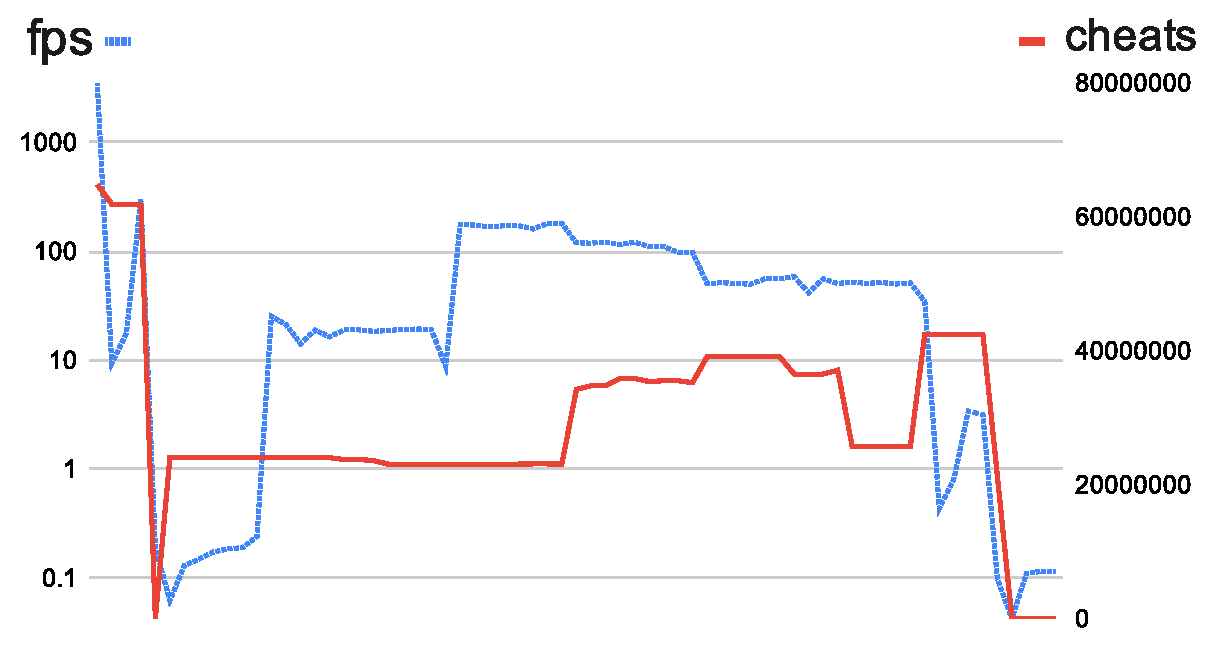
\includegraphics[width=0.95 \linewidth]{fpscheats}
  \caption{
    During the development of the emulator, the FPS achieved (blue) versus
    the number of times the code ``cheats'' due to incomplete implementation (red).
    Log scale. Honestly there's not much to get from this except that we start
    with a lot of FPS (3500) and a lot of cheats (65 million) and end with
    few FPS (0.1) and no cheats. I guess it also shows that this took many
    iterations to implement. The reason that cheats does not monotonically
    decrease is that a single cheat (e.g. a {\tt switch} on the instruction byte)
    can mask the need for hundreds of other cheats.
  } \label{fig:cheating}
\end{figure}

Another challenge is that the 2A03 has dozens of undocumented
instructions with mysterious behavior. Most of these are not used by
any game in my test suite, which means I run the risk of breaking one
of these instructions and not knowing. Some of these instructions are
very weird, since they are essentially the consequence of 6502
sub-units (designed for implementing other instructions) being
connected together in ways that are not motivated by useful behavior.
For example, the {\tt XAA} instruction ({\tt 0x8B}) bitwise-ORs the
{\tt A} register with {\tt 0xEE} (setting all but two bits), then ANDs
with the {\tt X} register, then {\tt AND}s with an immediate byte.
Others are just as weird but much more complex. Since I want the
emulator to be as complete and correct as possible, I wrote a new
``game'' that I could use as an additional test ROM
(Figure~\ref{fig:testrom}). This ``game'' executes dozens of
undocumented instructions at startup, writing interesting state to RAM
to create a record of their behavior. The game then displays the first
half of RAM on screen. This gives some amount of protection against
regression on these instructions.

\paragraph{Everything, everywhere, all at once.}
Each instruction is otherwise straightforward to implement. The
remaining challenge has to do with the instruction dispatch. A natural
way to write the instruction loop is to do {\tt switch} on the
instruction byte, but that is not a linear operation. Instead, we
always execute all of the instructions. Before this, we make 256
copies of the CPU state (the registers); this is linear because it's
just copying a finite number of variables. Each copy also has an {\tt
  active} flag (a {\it hfluint8} with $1$ or $0$). We set this for
exactly one of these instructions, by computing
\verb+If(Eq(insn_byte, n))+ for each of the 256 {\tt n}. Then we
execute each instruction on its copy of the state; it does all its
computation, and any read or write is additionally conditioned on
its {\tt active} flag.

We then need to select the instruction that was actually executed
and copy its state back to the ``real'' CPU state. We do this by
conditionally clearing each register:

$${\tt reg = If(active, reg)}$$

We then set the real CPU's register to the sum of all of the registers
from the instruction-specific states. Exactly one (the active one)
will be nonzero, so we get that value. We use this same technique to
keep track of how many cycles have elapsed, since various emulator
timing depends on this.

A bad thing about this approach is that it's more than 256 times slower
than just executing a single instruction, and this is the main reason
why the emulator is so slow. A good thing is that there is no cheating.
Another good thing is that the instructions are all reading and writing
distinct data, so they can actually be executed in parallel. The final
benchmarks here are from running on 8 cores.

\begin{figure}[htp]
  \begin{center}
    \includegraphics[width=0.9 \linewidth]{testrom}
  \end{center}
  \caption{
    Exciting Nintendo ``game'' showing the first half of the NES RAM after
    executing a test of dozens of undocumented instructions.
    The ``game'' cannot be won. It exists only to destroy your mind.
  } \label{fig:testrom}
\end{figure}

\subsubsection{It's a-fine, Mario!}

The emulator can play any NES game supported by FCEUX (which is
basically all of them; despite the horrors in this emulator's code, it
has great compatibility). My benchmark was the first level of the
classic {\it Super Mario Bros.}, playing sequence of 2210 inputs that
completes level \verb+1-1+ in 36 seconds. The emulator runs this as
fast (or as slow) as it can. Normal frame rate is 60~FPS. The original
implementation runs at 3500~FPS; after many performance tweaks I got
my {\it hfluint8} version to run at

$${\large 0.1154~\textrm{FPS}}$$

In print, the frame-rate is always zero, anyway
(Figure~\ref{fig:mario}). 8.6 seconds per frame is firmly in ``not
playable'' territory, but it is tolerable for installation artwork,
let's say. I have played AAA titles that, at launch, inexplicably had
comparable framerates on a high-end GPU, and these games were no doubt
executing a great many non-linear instructions.

\begin{figure}[htp]
  \begin{center}
    \includegraphics[width=0.9 \linewidth]{mario-1800}
  \end{center}
  \caption{
    Mario completing level {\tt 1-1} in 36 seconds of game time,
    or 19,143 minutes of wall time, using only floating point roundoff
    error from addition and scaling.
  } \label{fig:mario}
\end{figure}

\section{Conclusion}

Implementing a basic computer (with an extant software library) using
floating point addition and scaling demonstrates the highly general
computing power they contain, despite approximating mathematically
limited operations. We can say informally that they are Turing
complete. This also renders the previous sections moot; performance
notwithstanding, we could directly implement the Mandelbrot set, the
{\tt tanh} transfer function, or AES using this 8-bit computer. It
also immediately gives us a linear chess engine (including game tree
search and a user interface) by emulating {\tt chessmaster.nes}; in
fact this engine already participated in our tournament
(Figure~\ref{fig:elo})!

\subsection{Future work}

If I remember correctly (and I probably don't), Go\"edel showed that
an axiomatic system with addition and multiplication can encode
sufficient facts about the natural numbers to engender {\it
  incompleteness}~\cite{goedel1930incompleteness}. However, a system
with only addition (such as Presburger arithmetic) does not have this
problem. Incompleteness is similar to the halting problem for {\it
  Turing complete} systems; in that it is easy to encounter given a
small set of primitives and the canonical demonstration is a
diagonalization argument. Is floating point addition alone Turing
complete? Can we prove it? If so, is the fact that real mathematical
addition and multiplication have this deep incompleteness property
related to the fact that IEEE-754 multiplication have the deep
computational property?\footnote{No.} Coincidence?!\footnote{Yes.}

If not addition alone, the FMA (fused multiply-add) instruction very
likely suffices, as it performs both a multiplication and addition.
This makes sense, as the equation $F = MA$ is fundamental to physics.

Thinking about the 2A03 implementation, each loop executes the exact
same set of instructions, with a high degree of parallelism. The use
of condition codes mimics the way that VLIW machines and modern GPUs
execute data-parallel programs. This seems to lend itself to highly
parallel execution on GPUs; in fact the ``Tensor cores'' designed for
accelerating ML inference can likely execute these floating-point
operations. Moreover, since the operations being executed are linear,
the entire computation is trivially differentiable. This means that,
if you don't think about it too hard (but you need to think about it a
medium amount of hard, because it is a confusing thought), you could
use NES instructions as transfer functions in a network, and
back-propagate errors (giving an error vector towards a machine state
and controller inputs that would yield the desired output state). This
of course would not actually work, similar to how automatic
differentiation does not actually work.

Other applications of this technology are possible, and further study
is warranted. For example, a common act in video editing is to
rearrange clips from a source video in alphabetical
order~\cite{murphy2014arst}. It was formerly believed that this
required non-linear video editing (aside from ``Already Being Filmed
In Lexicographic Order Type Videos''). But it seems straightforward to
use techniques from this paper to perform them linearly.

\subsubsection{Conclusion Conclusion}
A line has been drawn in the sand. The professor has been defeated. The dead horse has been beaten.
The paper is finally over.

\bibliography{grad}{}
\bibliographystyle{plain}

\end{document}
